\Chapter{REVUE DE LITTÉRATURE}\label{sec:RevLitt}
% Texte / Text.

\section{Robot logiciel développeur}\label{robot_logiciel_developpeur_revue}
% TODO faire une intro à la revue littéraire 
% Le chapitre 2 présente une revue de littérature concernant le terme de robot logiciel développeur, la génération de code, les logiciels libres et open source, la sécurité en lien avec le développement logiciel, la complexité du développement de ERP, le DevOps, les interfaces logiciel no-code / low-code, la création de communauté et la poïèse. 
%MODIFIER légèrement la phrase pour qu'elle soit un reflet de chaque revue dans ce chapitre, faire une phrase d'intro pour chaque article et un phrase critique à la fin. SI PAS LE TEMPS, faire les plus pertinents selon ta recherche. SUPER IMPORTANT mettre un paragraphe à la fin de la revue littéraire qui résume et qui dit pourquoi tout ça est en relation avec ta recherche. Mettre ce qui manque dans l'article en lien avec ta recherche.

Dans ce mémoire, le terme robot logiciel revient à quelques reprises, ainsi sa définition est «agent intelligent programmé afin d'imiter les capacités d'un être humain dans un système informatique ou afin d'effectuer un ensemble de tâches prédéterminées de manière automatique.»~\cite{robot_logiciel_oqlf_2018} Les autres termes suggérés sont «robot informatique» et «robot». Ainsi, un robot logiciel codeur est une intelligence artificielle orientée au développement logiciel. En anglais, il pourrait être nommé un «DevBot»~\cite{8823643}.

Selon les auteurs Erlenhov et al. en 2019~\cite{8823643}, le robot logiciel développeur idéal est un développeur de logiciels artificiel qui est autonome, adaptable et possède des compétences techniques ainsi que sociales. La référence à l'aspect social d'un robot logiciel développeur est, par exemple, l'outillage aux développeurs autour d'un éditeur asynchrone en temps réel tel que CodeBuddy~\cite{10.1145/3287324.3293750} ou CodePilot~\cite{10.5555/1030453.1030540} dans leur développement collaboratif.

\section{Génération de code}

Utiliser un générateur de code dans un contexte d'application web est efficace, comme le démontre les auteurs Uyanik et al. en 2020~\cite{SAHIN2020}, ils obtiennent un gain de performance en temps de développement de 98.95\% et 0 bogue via le générateur de code.

Dans un autre projet de les auteurs Pichidtienthum et al. en 2021~\cite{9436754}, en ajoutant une interface LCNC sur un générateur de code sur Odoo, ils obtiennent 20\% de réduction de temps pour le développement de module, puis des utilisateurs non développeurs peuvent utiliser cet outil pour faire des modules. Cette recherche est similaire à celle expérimentée dans ce mémoire, en excluant l'aspect de la rétro-ingénierie qui est manquante.

\section{Logiciel Libre et Open Source}

Le partage de bibliothèque Open Source est une méthode utilisée pour accélérer le développement permettant la réutilisation de code. L’Open Source permet aussi de supporter l'interopérabilité~\cite{open_interop_2011}, qui est la capacité de différents logiciels d'interagir et communiquer efficacement entre eux, de manière transparente et harmonieuse, sans entraves ni obstacles, même s’ils ont été développés par différentes organisations.

D'ailleurs, comme le mentionne les auteurs Hertel et al. en 2003~\cite{HERTEL20031159}, un des facteurs de motivation important est la perception de l'indispensabilité de ses propres contributions dans une équipe, associée à une évaluation élevée des objectifs de l'équipe et un fort sentiment d'auto-efficacité personnelle. Le générateur de code ne doit pas remplacer l'utilisateur, il doit l'accompagner dans son développement.

% \section{Logiciel Libre}
% Le logiciel libre entrave l’interopérabilité seulement pour les systèmes non compatibles avec la copyleft. Bien qu’elle prône la liberté du code, elle est restrictive.

% Cette restriction est nécessaire à la protection du développeur et de la communauté. 

\section{Sécurité}

Bien qu'il y a plusieurs aspects de sécurité à considérer, ce qui nous intéresse, ici, est la sécurité logicielle via son développement et ses dépendances.

Thompson démontre en 1984~\cite{thompson_trusting_1984} qu'il est possible d'injecter du code malveillant dans les outils de compilation d'un logiciel pour créer une faille de sécurité dans l'exécutable. Shah explique dans son blog en 2020~\cite{discussion_reflection_trusting_2020}, que la morale est assez simple : il est impossible de fonctionner\footnote{D'utiliser et d'avoir confiance sur des technologies} sans faire confiance à quelqu'un. À moins que vous n'ayez écrit tout le code vous-même, vous devrez faire confiance à la sécurité d'une partie du processus de traitement du programme.

Hors, s'il est nécessaire de faire confiance, comment peut-on faire confiance lorsqu'on observe des problèmes de compatibilité de licence libre~\cite{pfeiffer2022license}\cite{8667977}? Le développeur choisi des bibliothèques libres qui utilisent d'autres bibliothèques pas nécessairement libres et qui peuvent contenir des failles de sécurités~\cite{10.1145/3133956.3134048}, sans en être conscient. 

Pour revenir à l'article de Thompson, comme le mentionne Yona dans son blog en 2023, cela suggère que, tant que nous ne sommes pas en mesure de rétroconception\footnote{Faire de la rétro-ingénierie sur un développement.} et de contrôler pleinement la fonctionnalité des réseaux neuronaux, il existera un risque inhérent. Même si nous parvenons à résoudre le problème d'alignement et à rendre l'IA conviviale pour l'homme, les attaquants qui obtiennent un accès en écriture aux poids\footnote{Un poids est la valeur numérique d'une neurone dans un réseau de neurones.} pourront implanter leurs portes dérobées.~\cite{discussion_reflection_trusting_ia_2023}

Ainsi, il serait pertinent de développer un robot codeur qui soit en mesure de faire de la rétro-ingénierie sur une application et ses bibliothèques. Le générateur pourrait comprendre le fonctionnement de cette chaîne de dépendance et générer le code idéal pour la remplacer par une nouvelle application digne de confiances en validant la propriété intellectuelle libre.

\section{Les complexités de développer ERP}

L'auteur Pitetti mentionne en 2010 : «Le choix d’un ERP libre n’implique pas nécessairement une diminution des coûts dans la mesure ou le reengineering\footnote{Ré-ingénierie} n’a pas été correctement effectué[...] Un guide des bonnes pratiques permet d’éviter ces erreurs, de limiter les coûts du projet ou de se renseigner sur les différentes phases du projet»~\cite{pitetti2010implementation}. C'est pourquoi il est important de suivre les différentes étapes de réalisation du projet pour réduire les erreurs d'ingénierie sur le développement, voir Figure~\ref{fig:erp_implantation_cinq_etape} qui démontre un processus d'implantation d'un ERP en cinq étape proposé par l'auteur Braud en 2008~\cite{uqam_erp_benefice_2008}. À ce jour, les travaux du générateur de code viennent accélérer que la partie développement de ce processus, mais ils apporteraient un gain considérable si nous pouvons l'appliquer à toutes ces étapes.

\begin{figure}[htb]
\centering
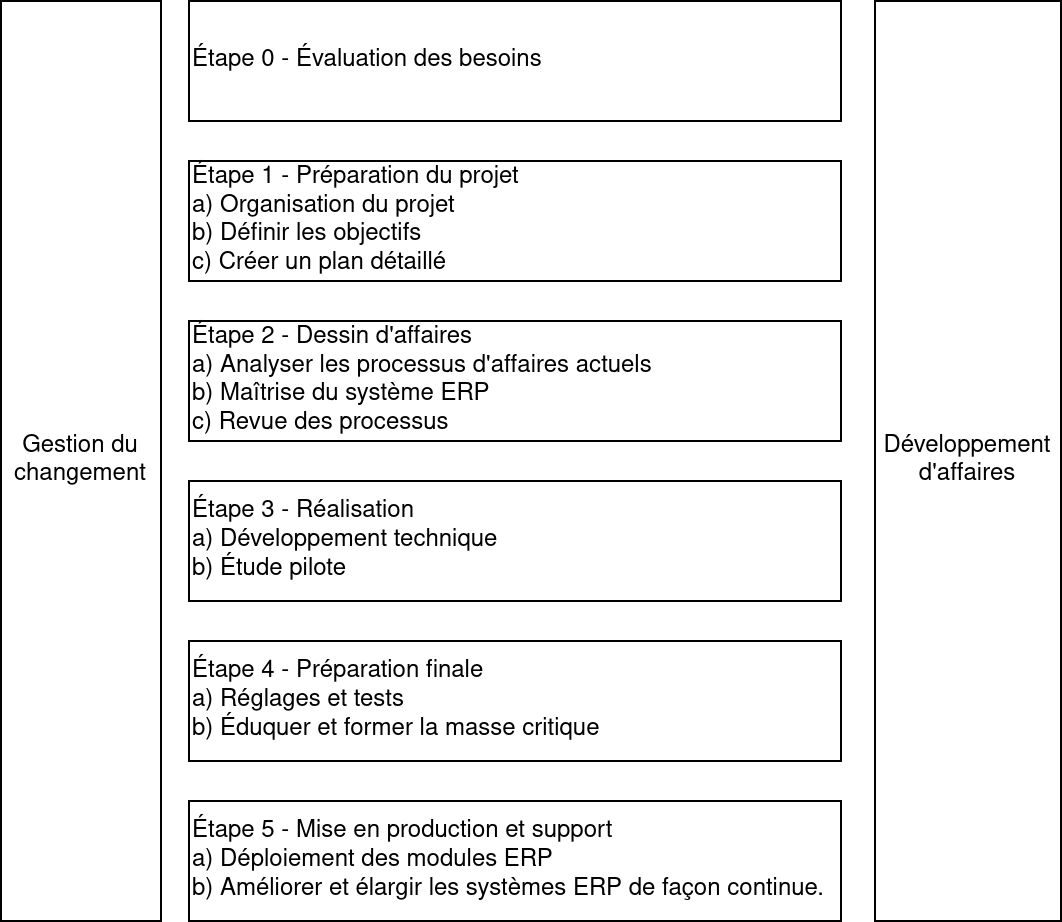
\includegraphics[width=4in]{processus_implantation_erp.drawio.png}
\caption{Processus d'implantation d'un ERP en cinq étapes. Image adaptée de l'auteur~\cite{uqam_erp_benefice_2008}}
\label{fig:erp_implantation_cinq_etape}
\end{figure}


Un autre facteur complexe est l'association des processus d'affaires actuels à la ré-ingénierie vers un nouveau modèle de processus d'affaires adapté aux contraintes technologiques, ainsi que les fonctionnalités déjà existantes sur la plateforme choisie. Comme on peut le constater dans le travail des auteurs Medjek et al. en 2018~\cite{kenza2018conception}, un travail a été effectué pour énumérer les fonctionnalités de la plateforme, ainsi que de faire du développement personnalisé avec tous les diagrammes de conception génie logiciel.

Dans Odoo, le nombre de module augmente avec le temps et diffère entre les versions, une recherche fastidieuse doit être effectuée pour réduire le temps de développement et à éviter de réinventer la roue. En plus de suivre toutes ces étapes, il faut mettre en place une pérennité pour l’amélioration continue sur le projet pour des adaptations futures aux nouveaux processus de l'entreprise.

% Autour de ça, il faut mettre en place une gestion du changement et adapter le développement des affaires.

% Plusieurs de ces étapes ne sont pas prises au sérieux, tel que le financement. De plus, l’implantation se fait sur une longue période de temps.

% Dans Odoo, le nombre de modules augmente avec le temps et diffère entre les versions, une recherche fastidieuse doit être effectuée pour réduire le temps de développement et à éviter de réinventer la roue.

% Il faut adapter les processus des organisations aux fonctionnalités existantes, sinon il est trop coûteux de tout recréer selon les processus de l’entreprise.

% En plus de suivre toutes ces étapes, il faut mettre en place une pérennité pour l’amélioration continue sur le projet, cela rend le processus lourd en plus de durer dans le temps.

\section{DevOps}\label{devops_ref}

Comme le mentionne l'auteur Ebert en 2016~\cite{ebert2016devops}, le DevOps consiste en un développement et une provision de processus commerciaux rapides et flexibles. Il intègre efficacement le développement, la livraison et les opérations, facilitant ainsi une connexion fluide et flexible de ces silos traditionnellement séparés, voir Figure~\ref{fig:devops}.

\begin{figure}[htb]
\centering
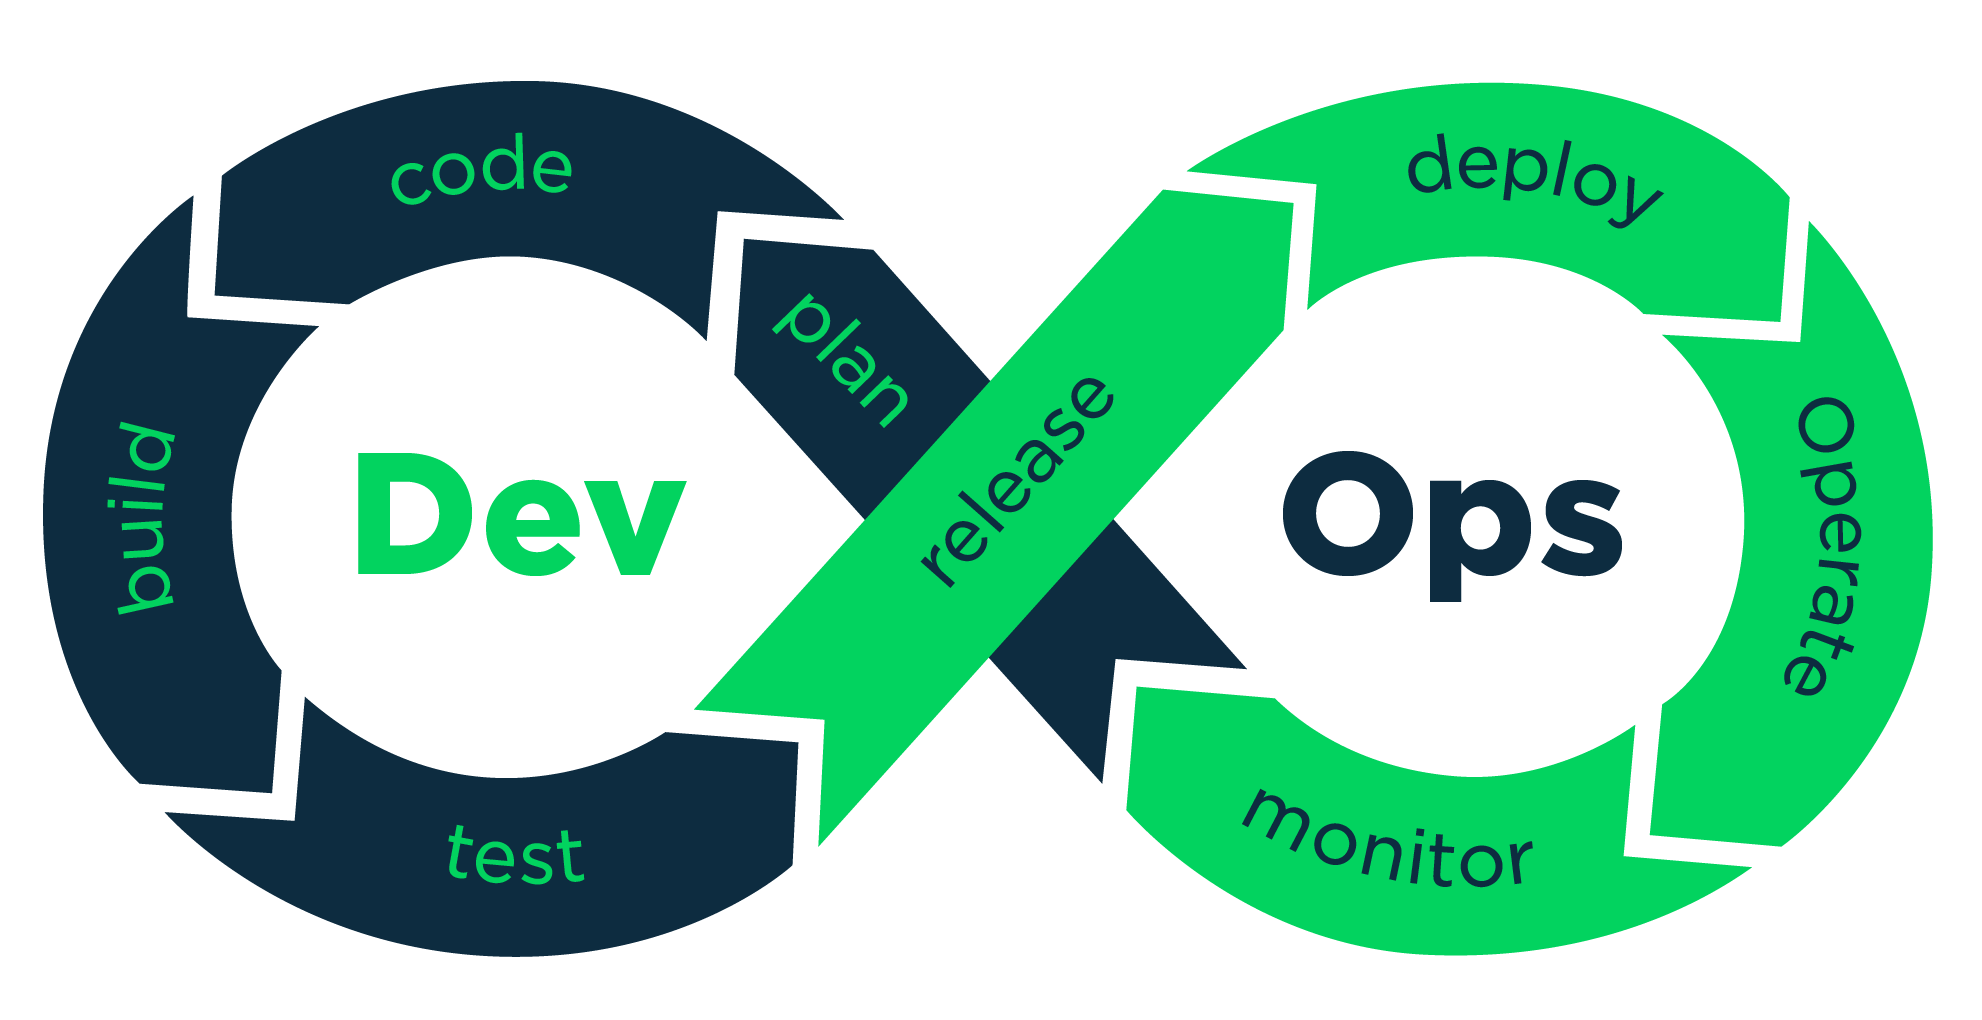
\includegraphics[width=4in]{devops.png}
\caption{Le processus DevOps. Source: Pease, 2017.~\cite{devops_illustration}}
\label{fig:devops}
\end{figure}


\section{Logiciel no-code / low-code}

% Basé sur des templates de code et une interface qui, au besoin, permet la configuration par du code.

Le LCNC est un concept qui permet à l’utilisateur de développer une plateforme ou des segments d'application en utilisant peu ou pas de code. Selon l'auteur Bock en 2021~\cite{LC_bock_2021}, la Figure~\ref{fig:lcnc_plateform} défini un ensemble des fonctionnalités nécessaire pour une plateforme LCNC. Les travaux de ce mémoire supporte : la gestion des rôles; un mécanisme de déploiement et exportation; un mécanisme pour changer le design de l'interface utilisateur; un mécanisme pour coupler l'interface à un modèle et un contrôleur (MVC); un mécanisme pour faire le rendu visuel sur différents types d'appareils; une gestion des processus du système et de la machine; un système de gestion des états et des transitions; un mécanisme de spécification fonctionnel de base; un générateur de code de composantes; un mécanisme d'accès à des API externes; des composantes de conception d'un modèle de données; des composantes pour spécifier des structures de données; La gestion de base de données interne et externes par API. Ainsi, la plupart des composantes communes sont supportés dans ces travaux, cependant il manquerait un générateur d'algorithme et un générateur d'interface dédié au générateur de code, puis d'autres composantes moins importantes.

\begin{figure}[htb]
\centering
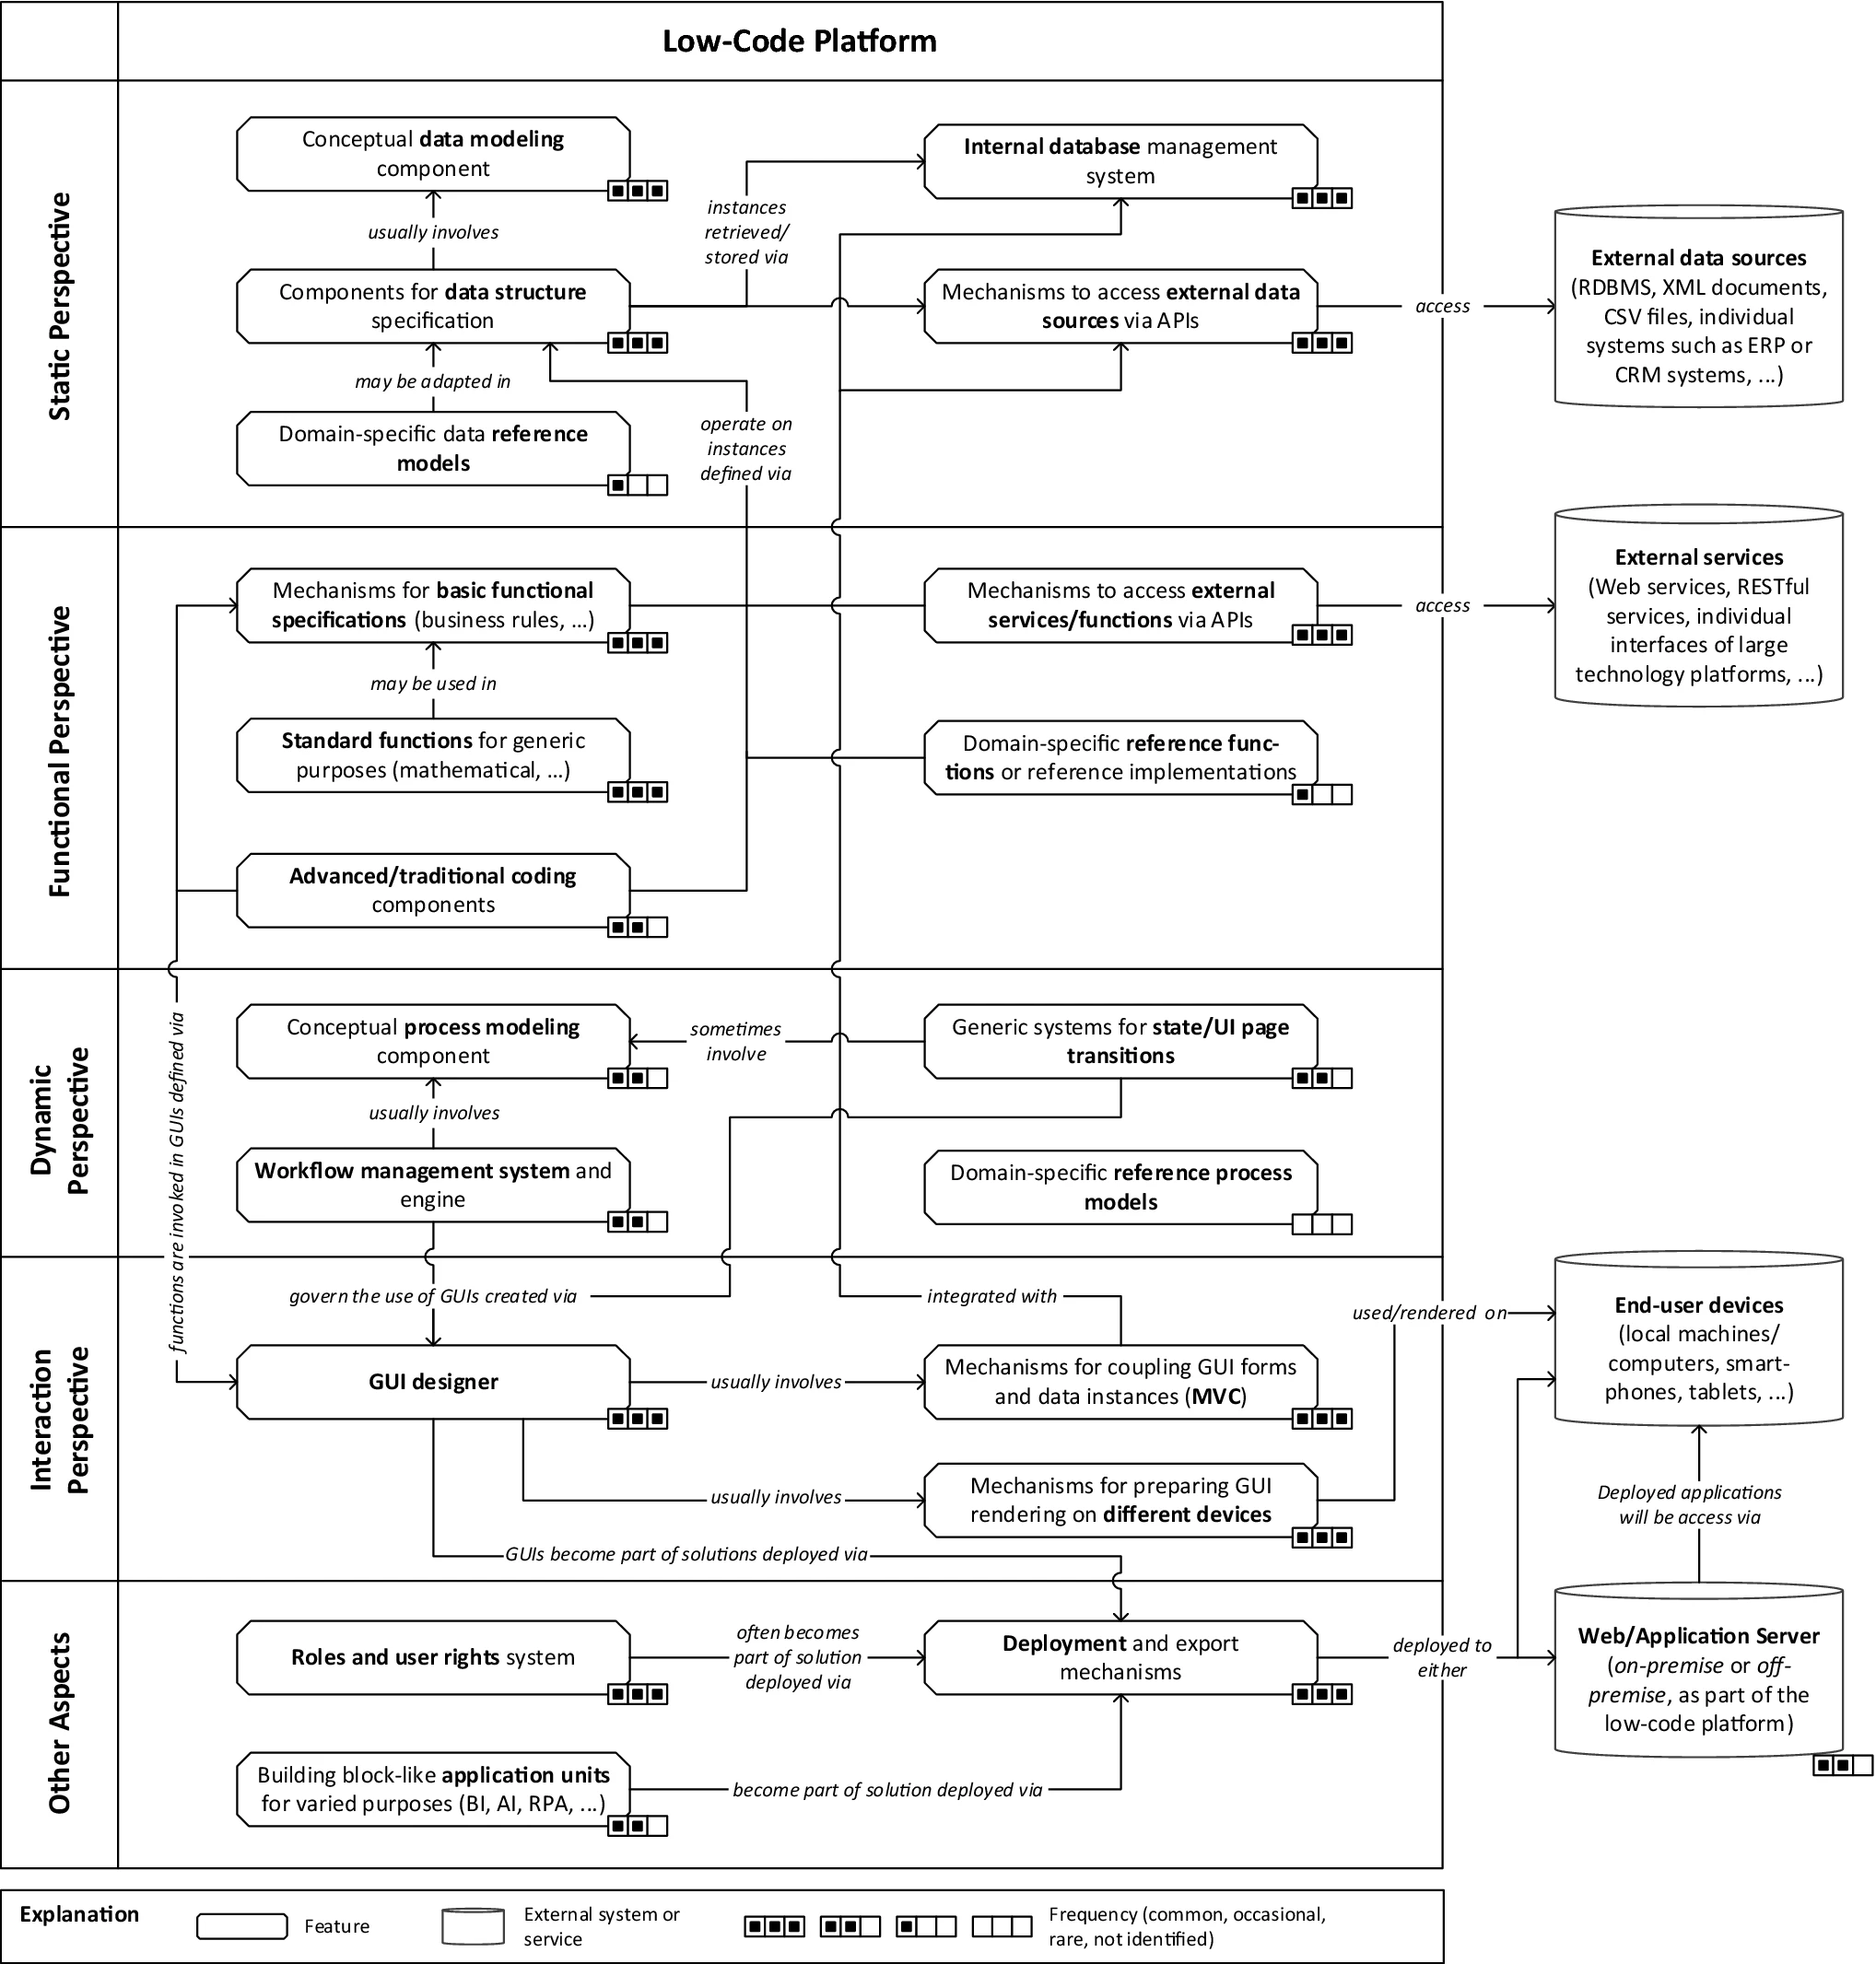
\includegraphics[width=5.5in]{12599_2021_726_Fig1.png}
\caption{Fonctionnalités des plateformes \textit{low-code}. Image provenant de~\cite{LC_bock_2021}}
\label{fig:lcnc_plateform}
\end{figure}

% \begin{enumerate}
%     \item Aspect général;
%     \begin{enumerate}
%         \item Gestion des rôles et permissions par des groupes utilisateurs ou individuelle;
%         \item Mécanisme de déploiement et exportation;
%     \end{enumerate}
%     \item Perspective d’intéraction;
%     \begin{enumerate}
%         \item Mécanisme pour changer le design de l’interface utilisateur;
%         \item Mécanisme pour coupler l’interface à un modèle et un contrôleur (MVC);
%         \item Mécanisme pour faire le rendu visuel sur différents types d’appareils;
%     \end{enumerate}
%     \item Perspective dynamique;
%     \begin{enumerate}
%         \item Gestion des processus du système et de la machine;
%         \item Composantes de modélisation de processus conceptuel;
%         \item Système de gestion des états et des transitions;
%     \end{enumerate}
%     \item Perspective fonctionnelle;
%     \begin{enumerate}
%         \item Mécanisme de spécification fonctionnel de base;
%         \item Générateur d’algorithme;
%         \item Générateur de code de composantes;
%         \item Mécanisme d’accès à des API externe;
%     \end{enumerate}
%     \item Perspective statique;
%     \begin{enumerate}
%         \item Composante de conception d’un modèle de données;
%         \item Composante pour spécifier des structures de données;
%         \item Gestion de base de données interne;
%         \item Gestion de base de données externes par API;
%     \end{enumerate}
% \end{enumerate}

Selon l'auteur Apurvanand en 2020~\cite{9226356}, voir Figure~\ref{fig:lcnc_plateform_dev}, pour mettre en place une plateforme de développement avec réduction de code, il est nécessaire d'avoir une base de données, des services externes, un répertoire de modèles réutilisable, une communauté de collaborateur, un compilateur, un optimisateur des requêtes, un générateur de code, un ensemble de service au développement (journalisation, déploiement, audit, versionnage de code), ainsi qu'une application visuelle pour tout produire tous les éléments nécessaire à l'application désiré. Dans les travaux de ce mémoire, tous ces éléments sont déjà accessibles, mais en début de maturité.

\begin{figure}[htb]
\centering
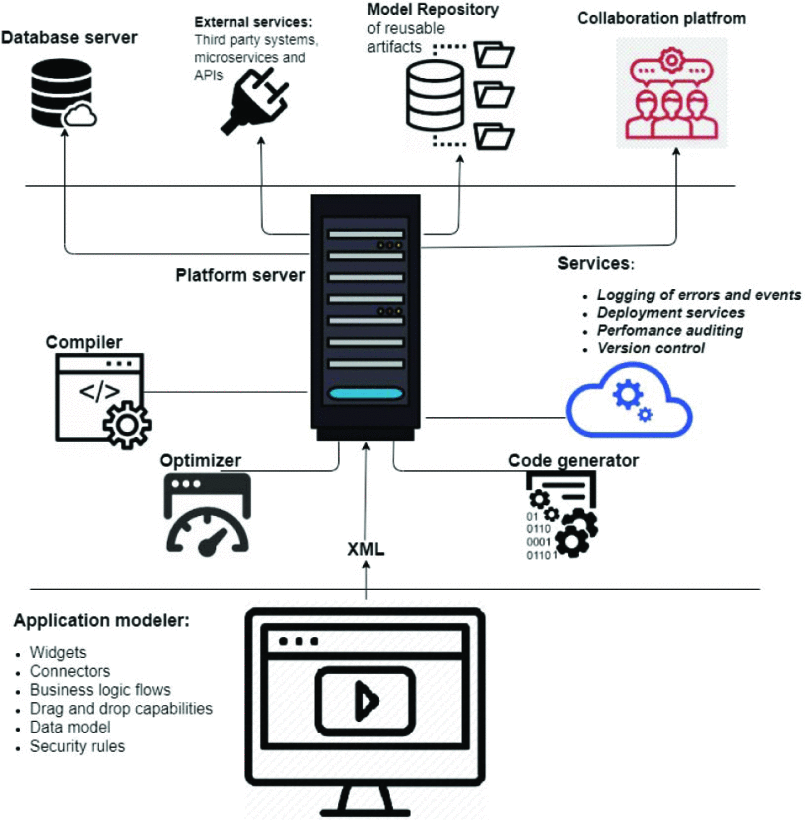
\includegraphics[width=4in]{sahay2-p8-sahay-large.png}
\caption{Les composantes principales d'une plateforme de développement \textit{low-code}. Image provenant de~\cite{9226356}}
\label{fig:lcnc_plateform_dev}
\end{figure}


% Selon l'auteur Apurvanand en 2020~\cite{9226356}, il faut les éléments techniques suivants pour supporter une plateforme LCNC :
% \begin{enumerate}
%     \item Bases de données;
%     \item Services externes;
%     \item Gestion des modèles de données;
%     \item Plateforme collaborative;
%     \item Service infonuage (déploiement, audit de performance, gestion des erreurs/traces/événements, gestion des versions);
%     \item Générateur de code;
%     \item Compilateur et optimiseur de code;
%     \item Modeleur d’application;
%     \begin{enumerate}
%         \item Widget;
%         \item Connecteur;
%         \item Processus de logique métier;
%         \item Capacité de «drag and drop»;
%         \item Modèle de données;
%         \item Règles de sécurité;
%     \end{enumerate}
% \end{enumerate}

% L'auteur Apurvanand poursuit en mentionnant les besoins de niveau supérieur d’une plateforme LCNC :
% \begin{enumerate}
%     \item GUI;
%     \item Interoperabilité, support entre services externes et base de données;
%     \item Support de la sécurité;
%     \item Support d’une plateforme collaborative;
%     \item Support sur la réusabilité, pouvoir répété l’utilisation d’une composante dans différents contextes;
%     \item Support de la capacité d’un système à maintenir ou à améliorer ses performances;
%     \item Mécanisme de spécification de logique du développement des affaires;
%     \item Logiciel pour construire des mécanismes;
%     \item Support au déploiement;
% \end{enumerate}

% Hors, en supportant l'ensemble de ces mécanismes et éléments techniques, nous devrions obtenir un LCNC intégré dans le robot logiciel codeur.

% \section{Dev ops}
% Démontrer outil
% TODO image dev ops

% La partie générateur de code répond seulement au besoin création de code du dev ops.

\section{Création d’une communauté}

% todomarie ----------------------------- TU DOIS INTRODUIRE LE CONCEPT DE COMMUNAUTÉ,CEST QUOI LE RAPPORT AVEC TON MÉMOIRE ET OU TON PROJET-----------
% VOIR LCNC dev, besoin de communauté

«Il est important de comprendre que les logiciels libres et ouverts sont soutenus et entretenus, non pas uniquement par un éditeur logiciel traditionnel mais également par une communauté constituée de ses utilisateurs, qu'il s'agisse d'éditeurs, de sociétés de services spécialisées ou d'utilisateurs. Ce sont ces communautés qui décident de l'orientation technologique, de l'adaptation et de l'évolution du code source ainsi que des versions et des mises à jour qui seront rendues disponibles. Un logiciel libre et ouvert évolue proportionnellement au dynamisme de sa communauté[...]»~\cite{tresor_gouv_logiciels_libres}

«La conviction selon laquelle la créativité d’un groupe est à la fois le fruit de l’autonomie et de l’engagement de ses membres commence à se diffuser au sein des sciences sociales. Le logiciel libre en offre un parfait exemple ; c’est un logiciel dont le code source est rendu ouvertement disponible et modifiable par tous : une fois publié, le code source n’appartient plus à son créateur et son évolution dépend de ce que les autres usagers en font.»~\cite{REDP_173_0387}

\subsection{Communication non violente}

La mise en place d’une méthode de communication non violente~\footnote{\url{https://fr.wikipedia.org/wiki/Communication_non_violente}} formalisée par Rosenberg en 2015~\cite{rosenberg2015nonviolent}, voir Figure~\ref{fig:communication_non_violente}, permettrait de réduire les frictions et faciliter l'intégration entre les participants du réseau d’entraide.

\begin{figure}[htb]
\centering
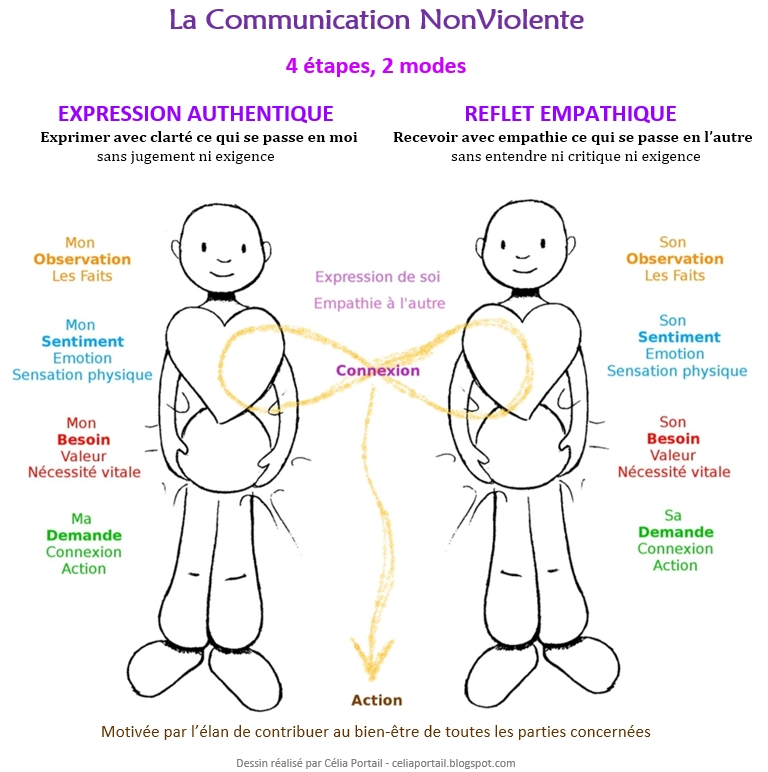
\includegraphics[width=4in]{OSBD_en_CNV.jpg}
\caption{Communication non violente en 4 étapes et 2 modes. Dessin réalisé par Célia Portail~\cite{wikipedia_image_non_violente}}
\label{fig:communication_non_violente}
\end{figure}

\subsection{Guide construire une communauté Open Source}

Un guide~\cite{url_open_source_guide} est accessible publiquement pour aider les gestionnaires de communautés en 4 sections avec des titres indicateurs d’orientation : la mise en place de votre projet pour le succès, cultiver votre communauté, résoudre les conflits et la communauté est le coeur de l'open source. Il y a beaucoup d'autres guides, mais en général, ils n'intègrent ni les aspects de génie industriel qui est vulgarisé avec le guide fusée et ni les critères éthiques de GNU concernant l’hébergement de logiciel.

% Il faut :
% \begin{enumerate}
%     \item rédiger un code de conduite;
%     \item proposer la contribution directement sur le projet.
% \end{enumerate}
% TODO supporter les autres pages https://opensource.guide/fr/metrics/

\subsection{Guide fusée}

Un guide en 7 étapes du guide Fusée de CimarLab en 2023~\cite{guide_fusee}, voir Figure ~\ref{fig:guide_fusee} pour les gestionnaires de projet. Il permet de démarrer un projet rapidement qui nécessite une équipe de personnes pour les rendre efficaces dans la réalisation de leur participation dans le réseau d’entraide.

\begin{figure}[htb]
\centering
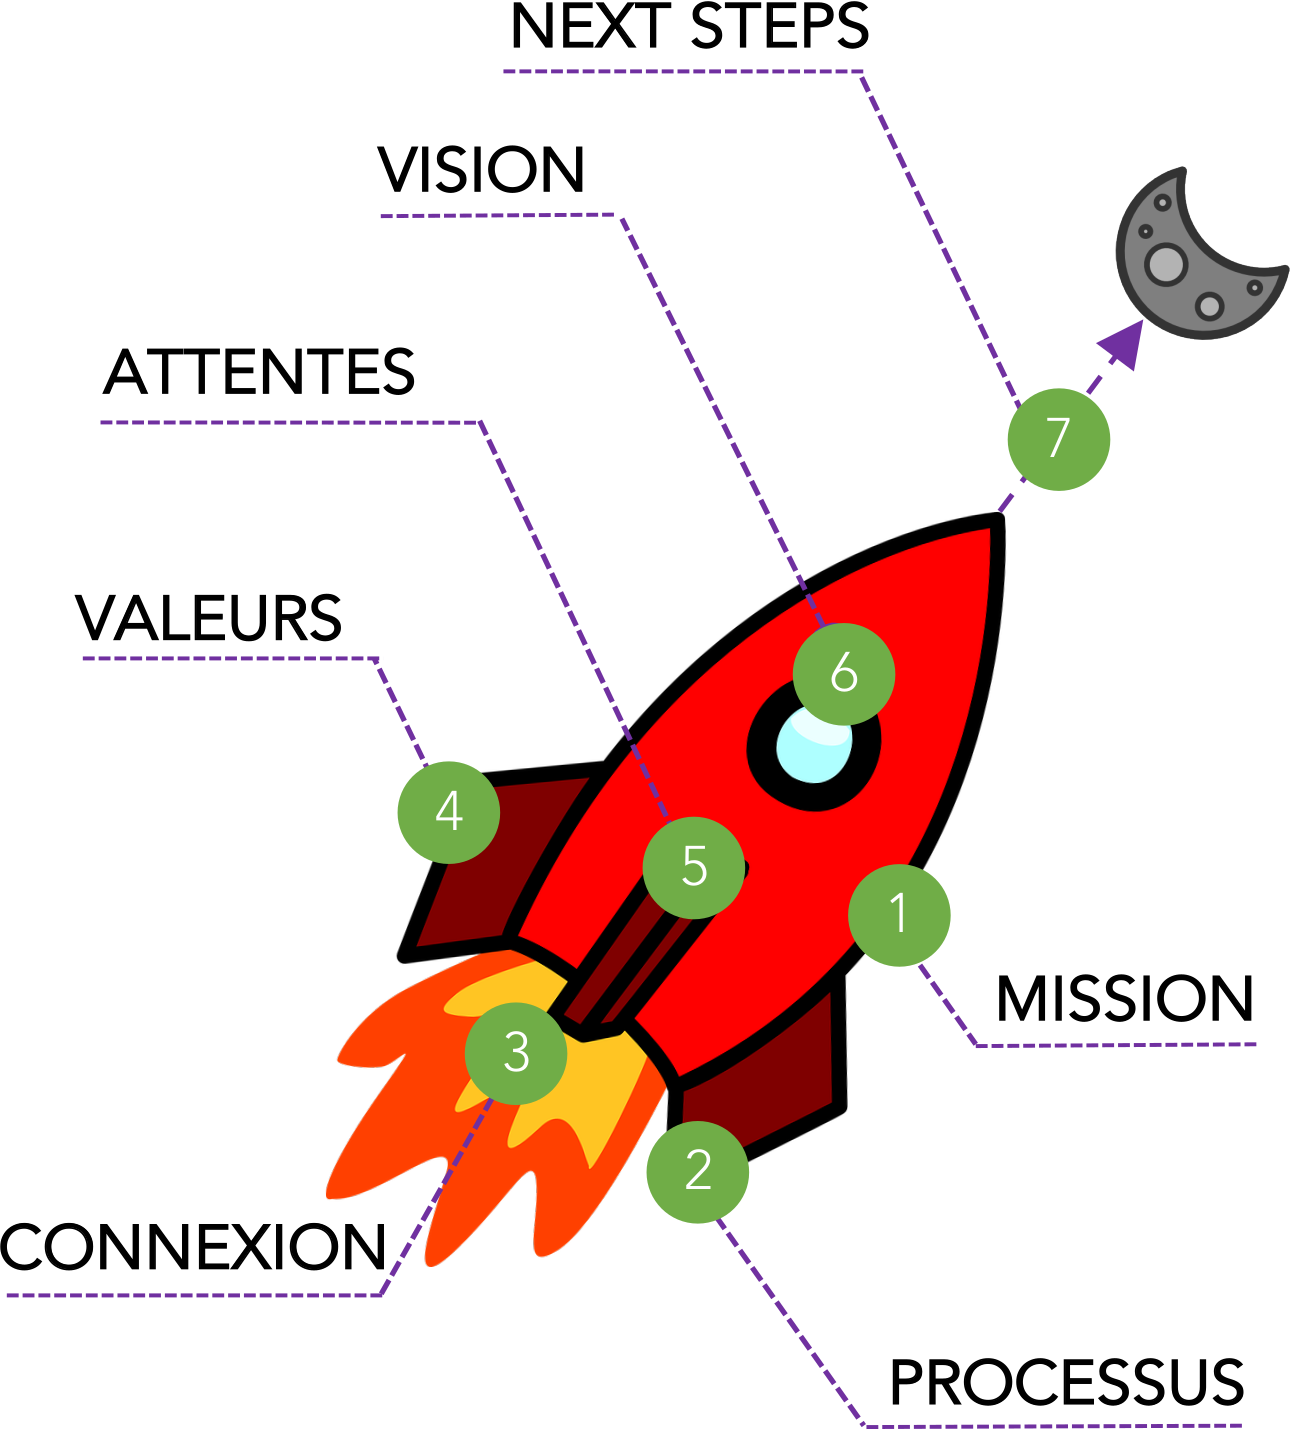
\includegraphics[width=2.5in]{guide_fusee_definition.png}
\caption{Guide fusée en 7 étapes pour démarrer un projet pour un gestionnaire de communauté, de CimarLab~\cite{guide_fusee}}
\label{fig:guide_fusee}
\end{figure}

\subsection{Critères éthiques de GNU concernant l'hébergement de logiciel}

La licence AGPLv3 n’est pas toujours bien respectée~\cite{violation_libre_2017}. Il est important d'assister le développeur dans ses choix de licence et compréhension des licences des bibliothèques tierces. Cependant, une fois que le logiciel est prêt à être mise en production, il y a des critères éthiques concernant l'hébergement de logiciel~\cite{gnu_critere_hebergement_2022} qui doit être accessibles sur les projets du réseau d’entraide. Un guide avec des critères mesurables pour les services destinés à tous ceux qui veulent utiliser un service pour héberger publiquement du code source libre, ainsi qu'éventuellement des programmes exécutables devra être mis à la disposition des organisations. Ces critères se concentrent sur la protection de la vie privée, le fonctionnement sans JavaScript non libre\footnote{\url{https://www.fsf.org/campaigns/freejs}}, la compatibilité avec les licences à copyleft et leur philosophie, et l'absence de discrimination contre les utilisateurs, quels qu'ils soient. 

% \begin{enumerate}
%     \item Est-ce que l'hébergeur fournit l'accès au code source des programmes qu'il héberge?
%     \item Est-ce que l'hébergeur permet la redistribution des copies des programmes qu'il héberge?
%     \item Est-ce que l'hébergeur permet aux utilisateurs d'apporter des modifications aux programmes qu'il héberge et de les partager avec la communauté?
%     \item Est-ce que l'hébergeur impose des restrictions sur l'utilisation ou la redistribution des programmes qu'il héberge?
%     \item Est-ce que l'hébergeur respecte les licences de logiciels libres et les droits d'auteur associés aux programmes qu'il héberge?
%     \item Est-ce que l'hébergeur fournit des informations sur les licences de logiciels libres et les droits d'auteur associés aux programmes qu'il héberge?
%     \item Est-ce que l'hébergeur respecte la vie privée et la sécurité des utilisateurs des programmes qu'il héberge?
%     \item Est-ce que l'hébergeur fournit un support et une assistance adéquats aux utilisateurs des programmes qu'il héberge?
% \end{enumerate}

\section{Poïèse}

\subsection{Définition de la poïèse}

La poïèse~\cite{wiktionary_poiese_2022} (ou poïesis) est un terme d'origine grecque qui désigne le processus créatif de fabrication, de production ou de création. Il est souvent utilisé dans le contexte de l'art et de la littérature pour décrire le processus de création d'une œuvre, que ce soit un poème, une pièce de théâtre, un roman ou une peinture.

Dans ce contexte, la poïèse est considérée comme un processus actif et dynamique, impliquant l'imagination, l'inspiration, la créativité et la maîtrise technique. Elle implique souvent un certain niveau d'engagement personnel et émotionnel de la part de l'artiste\label{poiese_artise} ou du créateur.

En dehors de l'art, le terme poïèse~\cite{wikipedia_poiese_2022} peut également être utilisé pour décrire tout processus de création ou de production, y compris dans des domaines tels que la science, la technologie ou l'industrie.

Les termes «Allopoïèse», «Autopoïèse», «Sympoïèse» ont été inventés pour décrire des phénomènes biologiques, hors dans ce mémoire, ils ont été adaptés pour un contexte technologique.

\subsection{Technopoïèse}

% Un système technologique qui développe. Caractéristique d'une technologie qui fait de la poïèse.

% Un système technologique qui travaille pour la poïèse en mettant en place plusieurs caractéristiques, par exemple : l'«Allo» et l'«Auto».

La technopoïèse peut être décrite comme un système qui développe une technologie.

La technologie est là pour assister l'utilisateur et l'accompagner dans l'évolution de celle-ci. «Parce que l’appareil prend place entre la manifestation de l’œuvre et le travail de l’artiste en les découplant, en leur imposant une langue intermédiaire qui code puis décode. L’artiste produit des lignes de code, que la technologie intègre pour fournir à l’œuvre la source de sa manifestation : elle sépare ontologiquement\footnote{Une ontologie est une représentation formelle et explicite de la connaissance d'un domaine, qui spécifie les concepts, les relations et les entités qui existent dans ce domaine et comment ils sont interconnectés.} le travail de l’un et son résultat dans l’autre.»~\cite{artiste_techno_conf_2012} L'artiste~\footnote{Voir l'artiste de la «Définition de la poïèse»~\ref{poiese_artise}} ici signifie un programmeur informatique dans un processus créatif de fabrication, de production ou de création sur des technologies.

Pour éviter que la machine ne prenne le dessus, il faut l'orienter vers la technopoïèse. «Si la technologie est un médium parasite, alors ne suffit-il pas de compter sur la charge poïétique du médium primaire, pour conserver à la poïèse ses caractères nécessaires – et imaginer l’art technologique comme un art d’abord, agrémenté, partiellement seulement, de technologie?»~\cite{artiste_techno_conf_2012} % Cette machine doit être libre pour respecter l'humain. % TODO référence machine libre respect humain

%«Our main claim in this study is to underline that the biopoetic process organizing technopoiesis involves at least four levels, with emergences and constrains between the levels. Furthermore, we see technopoiesis as the dynamics between these four levels based on mechanisms expressing the relation between biology, poetics and external representations that cognitively and socio-culturally ground the evolution of technology.»~\cite{10553_41343}

Ainsi, le terme «technopoïèse» fait référence à la capacité de l'humanité à créer et à façonner la technologie pour répondre à ses besoins et à ses désirs. La relation entre la sympoïèse et la technopoïèse permettrait de concevoir des technologies plus durables et écologiquement responsables, qui favorisent la production collective et collaborative dans les écosystèmes. 

\subsection{Allopoïèse}

L'Allopoïèse peut être décrite comme un système qui développe\footnote{production/fabrication : Utiliser sans limitation, Modifier pour adapter, Étudier pour comprendre le fonctionnement et Copier pour reproduire.} quelque chose avec des composantes externes.

Sur Wikipédia, «L'allopoïèse est le processus par lequel un système produit quelque chose qui n'est pas le système lui-même. Ceci est le contraire de l'autopoïèse.[...] La plupart des processus de production industrielle sont allopoïétiques : une chaîne de montage peut produire des voitures mais pas les machines utilisées dans cette forme de production. [...] La reproduction n'est pas une auto-production.»~\cite{wiki_allopoiesis_2018}~\cite{vuc_allopoiesis_2018}

% «une définition qui est proche de celle d’une machine abstraite et qui décrit la machine comme autopoïétique, autoproductrice d’elle-même et reproduisant en permanence ses composantes tel un système sans input ni output. Varella développe assez loin cette théorie. Il oppose dans sa conception, l’autopoïèse qu’il rapporte essentiellement aux êtres vivants biologiques, à une allopoïèse où la machine va chercher ses composantes à l’extérieur d’elle-même. En fait, dans son concept d’allopoïèse il range les systèmes sociaux, les machines techniques et, pour finir, tous les systèmes machiniques qui ne sont pas des systèmes vivants.»
% «Les machines allopoïétiques se trouvent toujours en adjacence à des machines autopoïétiques et il faut donc prendre en considération les agencements qui les font vivre ensemble.»
% Citer ce document / Cite this document :
% Guattari Félix. À propos des machines. In: Chimères. Revue des schizoanalyses, N°19, printemps 1993. pp. 85-96 ;
% doi : https://doi.org/10.3406/chime.1993.1881
% https://www.persee.fr/doc/chime_0986-6035_1993_num_19_1_1881


\subsection{Autopoïèse}

L'autopoïèse peut être décrite comme un système qui se développe par soi même avec seulement ses composantes internes.

«L'autopoïèse est la propriété d'un système de se produire lui-même, en permanence et en interaction avec son environnement, et ainsi de maintenir son organisation (structure) malgré son changement de composants (matériaux) et d'informations (données).[...]le maintien de sa propre organisation (auto-production)»~\cite{wiki_autopoiesis_2022}.

Le maintien de sa propre organisation signifie l'auto-production, voir exemple illustratif auto-reproducteur du code~\ref{exemple_illustratif_auto_reproducteur}.

Selon l'auteur Nomura en 2000~\cite{tatsuya_computational_autopoiesis_2000}, un système est de l'autopoïèse dans le contexte qu'il est : 
\begin{enumerate}
    \item \textbf{Autonome} : il doit être capable d'apporter des changements variés pour maintenir son organisation;
    \item \textbf{Individuel} : il doit être indépendant dans sa définition, par sa prise de décision par rapport aux observateurs externes, en reproduisant à répétition et en maintenant son organisation;
    \item \textbf{Connaissant et établis ses limites} : il doit être capable d'établir ses limites dans son processus de reproduction par lui même sans se faire affecter des limites établis par les observateurs externes;
    \item \textbf{Absent d'entrant et de sortant} : Les stimulis externes doivent être interprété dans un contexte d'observation pour en retirer de l'amélioration continue, elles ne doivent pas impacter la maintenance de l'organisation directement, mais son évolution doit en prendre compte.
\end{enumerate}

Le concept de vue sur les entrants et sortants d'un système est une perception des observateurs externes et ne clarifie pas l'organisation ou les opérations de production du système. 

% TODO à valider : Ainsi, le système va opérer sans s'ajuster lui-même en rapport avec son état et le stimulis externe.

% TODO Alors comment fait-il pour se produire lui même en interaction avec son environnement s'il n'a pas d'entrant et sortant?

La conception d'un système autopoïèse, de l'article~\cite{tatsuya_computational_autopoiesis_2000}, devrait comporter les points suivants : 

\begin{enumerate}
    \item Les composantes du système sont déterminés par les opérations du système;
    \item Les opérations du système sont produites avant les conditions initiales;
    \item Les opérations du système sont seulement exécutées pour leur propre réussite et non pour réaliser la production d'un produit;
    \item Dans les opérations du système, ce qui se passe à l'intérieur du système est clairement différent des jugements des observateurs externes.
\end{enumerate}

% TODO La Technopoïèse doit être différent de l'autopoïèse, bien qu'il doit être autonome dans son évolution, il doit suivre des principes moraux et respecter des règles de société.

%  L'autopoïèse s'applique aussi à l'être humain, tant en sociologie\footnote{\url{https://fr.wikipedia.org/wiki/Sociologie}}, la science cognitive\footnote{\url{https://fr.wikipedia.org/wiki/Sciences_cognitives}}, la philosophie\footnote{\url{https://fr.wikipedia.org/wiki/Philosophie}} et la psychopathologie\footnote{\url{https://fr.wikipedia.org/wiki/Psychopathologie}}.

Appliquer l'autopoïèse sur un système est de forcer un changement de point de vue vers l'intérieur du système, puisque l'extérieur est matière à interprétation par la distinction de son environnement. En sciences naturelles, ce changement de point de vue est difficilement acceptable puisque le point de vue est fait par des observateurs externes.

Des modèles mathématiques sont expliqués dans l'article~\cite{tatsuya_computational_autopoiesis_2000} tel un système de réparation du métabolisme ((M,R) systems), introduit par Rosen, pour démontrer le «Quasi-Autopoietic Systems».
Puis il y a des modèles d'apprentissage automatique qui ont été inspirés de l'autopoïèse pour effectuer des tâches de reconnaissance de formes. Pour pouvoir représenter l'autopoïèse en mathématique ou en modèle informatique, il est nécessaire de trouver un mécanisme d'un système qui crée son espace avec ses limites et son environnement, par soi-même.

% TODO documentation intéressante : https://www.researchgate.net/publication/228784157_A_Computational_Aspect_of_Autopoiesis

\subsection{Sympoïèse}

La sympoïèse peut être définie comme un système qui se développe en collectivité. C'est un concept utilisée en écologie et en théorie des systèmes pour décrire les processus de production collective et collaborative dans les écosystèmes. Elle se distingue de l'autopoïèse, qui est le processus par lequel un système produit et reproduit ses propres composants de manière autonome. Par exemple, les coraux sont des collectifs d'organismes en interaction qui produisent des structures complexes telles que des récifs, qui ont des effets bénéfiques sur l'écosystème dans son ensemble.

Selon Guillibert en 2019, «La nature est une puissance d’engendrement qui surgit et s’autoproduit. Donna Haraway a récemment proposé de remplacer le concept "d’autoproduction" par celui de "sympoïèse" qui désigne la coproduction du milieu par des espèces en interrelations plutôt que l’activité autonome de certains organismes isolés.»~\cite{guillibert:tel-02929676}

Ainsi, le développement de technologie en collectivité va permettre de gérer des cas d'urgence humanitaire tel que le «mouvement des villes en transition»~\cite{MOUV_063_0130}\footnote{\url{https://fr.wikipedia.org/wiki/Ville_en_transition}} en développant des technologies permettant de mettre en place des systèmes d'échange local~\cite{cibois2010compte}\footnote{\url{https://fr.wikipedia.org/wiki/Systeme_d'echange_local}}.

% \subsection{Autotechnopoïèse}

% TODO source chatgpt

% L'auto-technopoïèse étend cette idée, de la technopoïèse, en suggérant que les systèmes technologiques peuvent devenir autonomes et se réguler eux-mêmes sans l'intervention humaine.

% L'autotechnopoïèse est un concept qui décrit la capacité des systèmes technologiques à s'auto-organiser et à s'autoréguler. Plus précisément, l'autotechnopoïèse se réfère à la capacité des systèmes technologiques à maintenir leur propre structure, leur fonctionnement et leur évolution, en utilisant des mécanismes internes de régulation et d'adaptation.

% Le terme "technopoïèse" fait référence à la capacité de l'humanité à créer et à façonner la technologie pour répondre à ses besoins et à ses désirs. L'auto-technopoïèse étend cette idée en suggérant que les systèmes technologiques peuvent devenir autonomes et se réguler eux-mêmes sans l'intervention humaine.

% Un exemple d'auto-technopoïèse est l'Internet, qui est un système complexe de réseaux informatiques interconnectés à l'échelle mondiale. L'Internet est capable de s'auto-réguler et de s'adapter à des changements dans son environnement, tels que l'augmentation du trafic de données ou les pannes de serveurs. Cela est rendu possible grâce à des mécanismes internes de régulation, tels que les protocoles de communication standardisés et les systèmes de routage dynamique.

% En résumé, l'auto-technopoïèse est un concept qui décrit la capacité des systèmes technologiques à s'auto-organiser et à s'auto-réguler. Cette capacité est de plus en plus importante à mesure que les systèmes technologiques deviennent plus complexes et interconnectés.

% Pour faire des améliorations technologiques dans la société, sur des réseaux d'entraide, il faut orienter l'autotechnopoïèse dans de la R\&D~\cite{innovation_complex_social_system_2010} orienté aux besoins technologiques dans la gestion de cas d'urgence humanitaire, par exemple le «mouvement des villes en transition»~\cite{MOUV_063_0130}\footnote{\url{https://fr.wikipedia.org/wiki/Ville_en_transition}}, en lien avec la sympoïèse.

% https://transitionlibre.ca

% Référence : 
% Teubner, G. (1993). Autopoietic law: A new approach to law and society. Walter de Gruyter.
% Luhmann, N. (1986). The autopoiesis of social systems. John Wiley & Sons.
% Castells, M. (1996). The rise of the network society. Blackwell Publishers.
% Ahrweiler, P. (2012). Innovation in complex social systems. Routledge.

\section{Définitions et concepts}


\subsection{Caractéristiques de la plateforme Odoo}

% TODO mettre les besoins issues des cas pratique (Accorderie) (CEPPP) et que les propriétés Odoo répondent à leur critère

\subsubsection{Architecture MVC}

Pour générer des modules Odoo, le générateur de code a besoin de s'appuyer sur l'architecture MVC pour permettre une séparation claire des responsabilités et une structure de code facile à maintenir. Le générateur doit ainsi générer chacune des sections de cette architecture pour faire un tout qui permet d'échanger les données entre la base de données et l'interface utilisateur.

L’architecture MVC permet de séparer les composantes logicielles par le modèle, la vue et le contrôleur. Le modèle représente les données et les règles de l’application. De plus, le modèle est responsable de la manipulation des données, de leur stockage et de leur récupération. La vue représente la présentation des données. De plus, la vue est responsable de l’affichage, à l’utilisateur final, des données stockées dans le modèle. Le contrôleur gère les interactions entre le modèle et la vue. De plus, le contrôleur est responsable de la réception des demandes de l’utilisateur et de leur transmission au modèle, puis de la récupération des données du modèle pour les transmettre à la vue. Il est possible de modifier une de ces composantes sans affecter les autres composantes, ce qui facilite la maintenance.

\subsubsection{Architecture ORM}

L'utilisation de requêtes SQL pour communiquer avec des bases de données demande un temps considérable au développeur à implémenter et elle nécessite la programmation d'interface avec la base de données. L'utilisation d'un ORM permet de bonifier la productivité, de faciliter la maintenance et d'augmenter la sécurité d'un logiciel. L’objectif du ORM est de faciliter la manipulation des données stockées dans une base de données relationnelle en les représentant sous forme d’objets dans un langage de programmation orientée objet\footnote{\url{https://fr.wikipedia.org/wiki/Mapping_objet-relationnel}}. Cela permet la simplification de l’architecture en l’écrivant en langage haut niveau, au lieu de directement en SQL, réduisant le nombre d'erreurs et facilite la maintenance.

\subsubsection{Architecture modulaire par héritage}

L'ensemble des fonctionnalités nécessaire à la gestion des procédures et ressources des organisations rend le développement complexe. Pour réduire cette complexité du développement logiciel, choisir une architecture modulaire permet la réutilisation de code et la création de relations fonctionnelles personnalisables au contexte des organisations.

L’héritage dans Odoo 12 peut se faire de deux manières : l'héritage par extension et l'héritage par substitution. L’héritage par extension permet d’ajouter des fonctionnalités ou de modifier le comportement d’un module existant, sans toucher au code source d’origine. Les nouvelles fonctionnalités peuvent être ajoutées en créant un nouveau module qui hérite du module d’origine et en y ajoutant des vues, des modèles ou des contrôleurs supplémentaires. L’héritage par substitution permet de remplacer complètement le comportement d’un module existant en créant un nouveau module qui hérite du module d’origine et en y modifiant les vues, les modèles ou les contrôleurs existants. En utilisant l’architecture modulaire avec héritage dans Odoo 12, les développeurs peuvent facilement personnaliser l’application pour répondre aux besoins spécifiques d'une organisation, sans toucher au code source d’origine et sans compromettre la compatibilité, par exemple, avec les mises à jour futures.

\subsubsection{Fonctionnalité du \textit{hook} lors de l’installation d’un module}

Au moment de l’installation d’un module Odoo, il y a des opérations qui peuvent être effectuées, comme migrer des données pour les adapter à un nouveau modèle de données. Ainsi, il y a une fonctionnalité qui se nomme le \textit{hook} pour «pre-install», «post-install» et «uninstall». Ce sont des méthodes qui sont exécutées soit au moment de l’installation, avant ou après l’initialisation de la plateforme, puis à la désinstallation. En «post-install», il devient possible d’exécuter du code et d'accéder à la plupart des fonctionnalités du ORM au moment d’installer un module. C’est une manière pour exécuter des scripts dans la plateforme au moment de l’installation d’un module, que ce soit en ligne de commande ou via l’application «Application» dans Odoo.

\subsubsection{\textit{Website builder}}

Le \textit{Website Builder} est un outil qui permet une autonomie aux utilisateurs lambda\footnote{Utilisateur semblable à la majorité dans son comportement. \url{https://fr.wiktionary.org/wiki/utilisateur_lambda}} (augmenter l'accessibilité) dans la création et mise à jour de contenus de pages web sur le site vitrine de l'organisation. C’est un mécanisme LCNC\footnote{Qui nécessite peu ou pas du tout du code} dans Odoo 12 pour créer et modifier un site web multi-pages par un mécanisme de \textit{drag and drop}\footnote{Glisser-déposer} avec des \textit{snippets}\footnote{Fragment de code} paramétrables. Il permet de modifier une page web en réduisant le besoin de recourir à un expert technique abaissant ainsi les coûts de développement.

\subsubsection{Internationalisation et localisation}

Il est nécessaire de supporter plusieurs langues pour faciliter la compréhension de l'outil informatique à l'utilisation. Pour y arriver, il existe un standard i18n, qui a été référencé \cite{i18n_wiley}, qui permet d'adapter les logiciels informatiques à plusieurs langues sur plusieurs localisations\cite{wikipedia_i18n}. Odoo rend accessible plusieurs bibliothèques pour permettre l’extraction de chaînes de caractères au moment de l’exécution, que ce soit dans du Python, Javascript ou XML. Le système permet de générer un fichier d'extension «.pot», qui contient ces chaînes de caractères. Pour supporter une nouvelle langue et une localisation, on copie le fichier d'extension «.pot» pour faire un fichier d'extension «.po» sous la nomenclature i18n et on peut faire la traduction ou l’adaptation linguistique. Le système peut aussi générer la langue existante pour faire un fichier d'extension «.po» avec les traductions déjà connues par le système, il suffit de le mettre à jour.

\subsubsection{ERPLibre}

Depuis la version 9.0 d'Odoo, une version communautaire et entreprise ont été créés causant une divergence sur les fonctionnalités, créant le modèle d'affaires «Open Core»\footnote{\url{https://fr.wikipedia.org/wiki/Open_core}}. L'adaptation d'un ERP est complexe et nécessite l'intervention d'experts pour bien répondre aux besoins de l'utilisateur pour la personnalisation de la plateforme aux réalités de l'organisation. Bien que l'OCA travaille pour rendre accessible librement ces fonctionnalités, cela vient limiter les réseaux d'entraide à pouvoir se débrouiller de manière souveraine.

La plateforme ERPLibre a ainsi été créée en début 2020 en encapsulant la version Odoo 12.0, sous licence AGPLv3, en offrant une alternative 100\% libre, dans le but de faciliter le déploiement et le développement pour une organisation en permettant la gestion des dépendances avec Poetry, automatisation du déploiement avec les Docker, la gestion de tous les répertoires de module~\ref{tab:nb_module_version_odoo} avec Git Repo\footnote{\url{https://gerrit.googlesource.com/git-repo}}, et plusieurs scripts pour le développement et une documentation propre pour son utilisation. Cela permet de rendre accessible, au même endroit, toute l'information nécessaire à la gestion de l'ERP d'une organisation.

% \subsection{Communauté de développement}

% % TODO manque why et how
% Une communauté de développement va regrouper une communauté de développeurs (qui travaille sur l’aspect technique) et une communauté d’utilisateurs (qui travaille sur l’aspect fonctionnel). Il faut réussir à faire interagir ces deux groupes d'individus et les amener à travailler ensemble.

% \subsubsection{Générateur de code accessible dans la communauté Odoo}

% % TODO REF
% % Il permet de générer un module simple dans Odoo et faire son modèle de données et vue de base admin

\subsection{Cadre conceptuel} \label{subsection_cadre_conceptuel}

Nous proposons un modèle formel de la génération de code qui guide le travail proposé dans ce mémoire. Soit C, un code informatique exécutable (qui pourrait aussi être un script interprétable), soit µ$_C$ les méta-données du code, et soit M, une machine disposant de deux modes d’opération : $M^d$ le mode direct, et $M^i$ le mode inverse, voir Figure~\ref{fig:mode_direct_inverse}. Lorsque M opère en mode direct sur µ$_C$, on doit obtenir C; en opérant en mode inverse sur C, on doit obtenir µ$_C$.

On peut représenter ces deux processus par les équations $M^d$(µC)=C et $M^i$(C)=µC. La machine peut alors être représentée par M = \{$M^d$,$M^i$\}.

L’ingénierie de génération est le mode direct. La rétro-ingénierie, le mode inverse, est le processus qui consiste à examiner et à analyser un système existant pour en comprendre le fonctionnement et les spécifications. Cette boucle va permettre d’intégrer des concepts d’amélioration continue sur l’évolution du code.

\begin{figure}[htb]
\centering
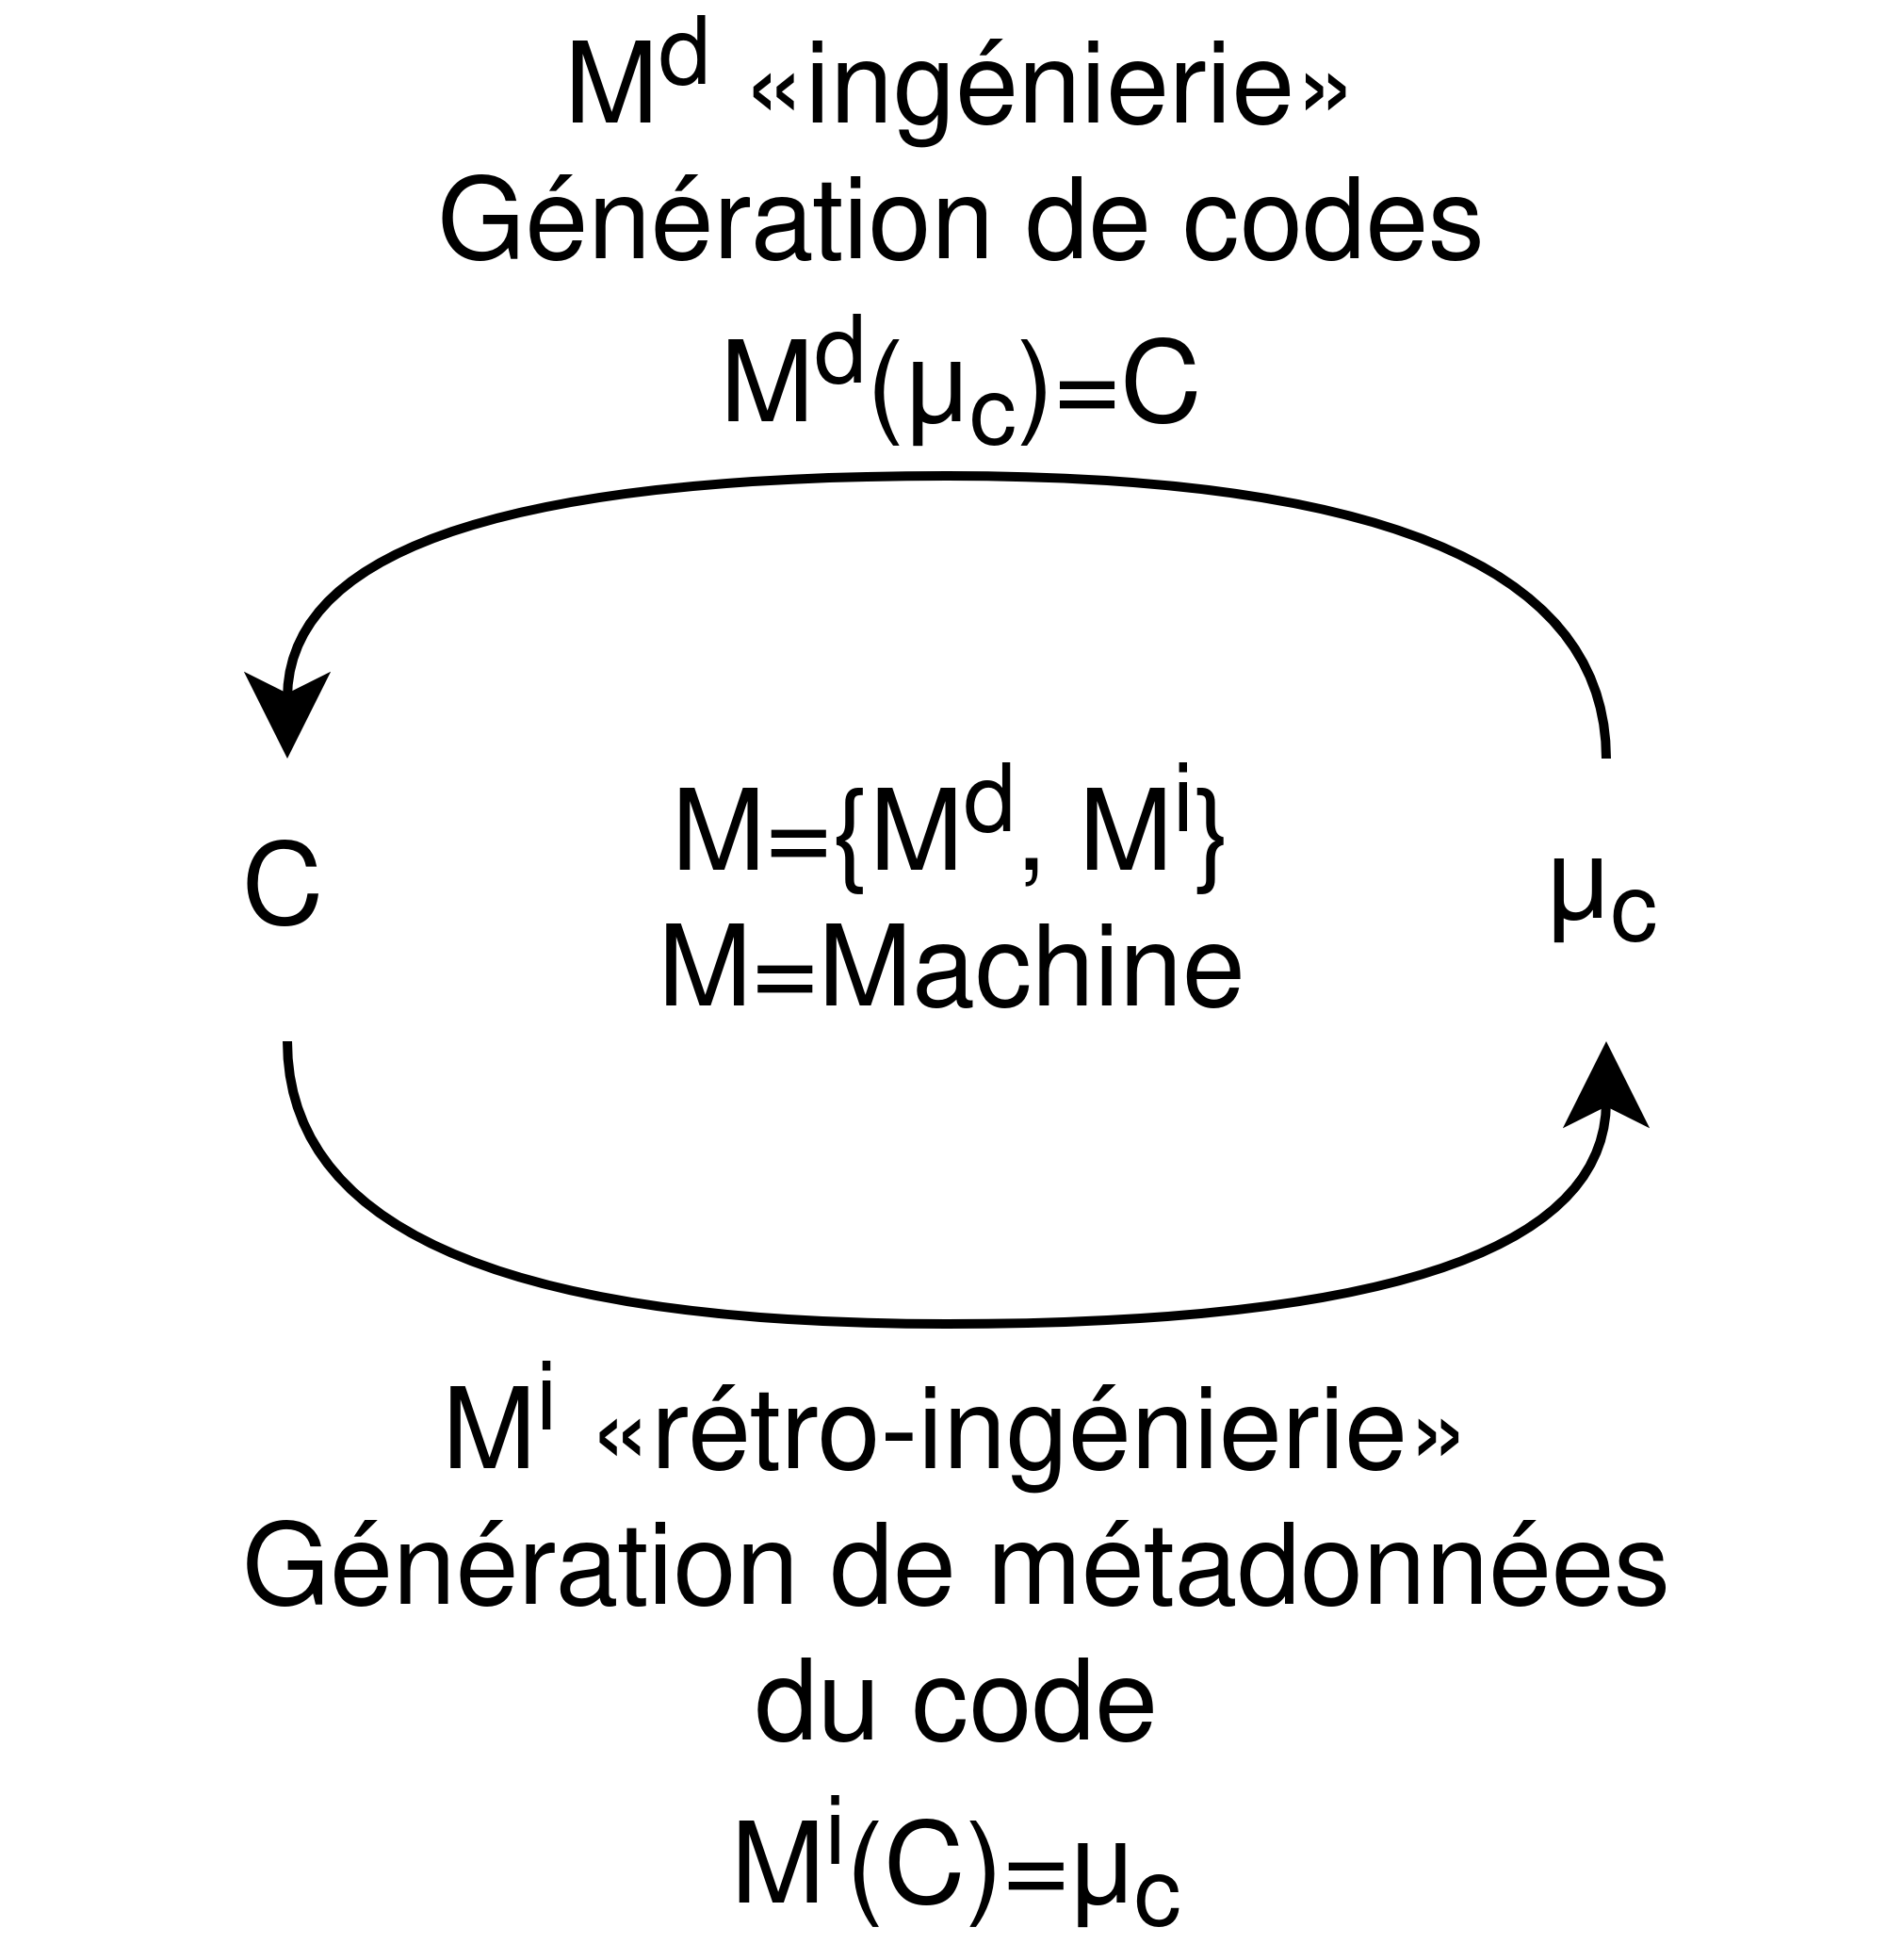
\includegraphics[width=2.5in]{images/machine_ing_retro_ing.drawio.png}
\caption{Mode direct et inverse}
\label{fig:mode_direct_inverse}
\end{figure}

Pour concrétiser le sens de ce modèle formel, nous allons proposer quelques exemples simples. Ayant pour but de faciliter la compréhension, ces exemples sont triviaux et ne présentent pas le plein potentiel de notre approche. L’interpréteur Python 3.6 et + est utilisé pour les exemples de codes.

Pour la plupart des exemples, le C, représenté par «C.py», est le code «Hello, World!», voir Figure~\ref{fig:exemple_code_hello_world}.

% \begin{lstlisting}[language=Python, upquote=false, caption={Exemple de code Hello, World!}, label={lst:exemple_code_hello_world}]
\begin{figure}
\begin{lstlisting}[language=Python]
print("Hello, World!")
\end{lstlisting}
\caption{Exemple de code Hello, World!}
\label{fig:exemple_code_hello_world}
\end{figure}

De plus, dans ce mémoire, nous utilisons le terme «générateur de code» qui est parfois représenté par «machine», cela fait référence à un ensemble de modules. Lorsque nous utilisons le terme robot logiciel codeur, nous faisons référence au «générateur de code» qui y est intégré, mais aussi à un ensemble de scripts dans ERPLibre, puisque le robot doit avoir un contrôle sur son projet en entier, jusqu'au déploiement de celui-ci. Ainsi, la machine est au niveau conceptuel théorique, le générateur de code est au niveau composante logicielle, et le robot logiciel codeur est au niveau de solution logicielle.

\subsection{Exemples illustratifs d’auto-reproducteur}\label{exemple_illustratif_auto_reproducteur}

\subsubsection{Le Quine}

«Un quine~\cite{sarkar2020quines} (ou programme auto-reproducteur, self-reproducing en anglais) est un programme informatique qui imprime son propre code source»~\cite{wiki_quine} sans se lire lui-même. Il doit contenir une logique d’écriture de code et contenir ses méta-données de génération. Il est ainsi un générateur de premier niveau.

Voir Figure~\ref{fig:exemple_quine}, la sortie textuelle dans la console, lors de l'exécution, est la même que son code.

\begin{figure}
\begin{lstlisting}[language=Python]
a='a=%r;print(a%%a)';print(a%a)
\end{lstlisting}
\caption{Exemple de code Quine}
\label{fig:exemple_quine}
\end{figure}

Cependant, le Quine ne sait rien faire d’autre que de s’auto-générer. Ce qui pourrait apporter une contribution serait de faire un auto-reproducteur qui permet de dériver vers d’autres fonctionnalités et ainsi intégrer l’amélioration continue sur son propre développement.

\subsection{Exemples illustratifs de générateur de code}

La génération de code est un des moyens pour soutenir le développeur dans le développement d’un logiciel. C’est la partie «création de code» de la méthodologie DevOps~\ref{devops_ref}.

\subsubsection{Technique de génération de code basique}

Dans Figure~\ref{fig:exemple_gen_code_basique}, la fonction «eval» en Python est dynamique, c'est-à-dire qu’elle permet l’exécution à partir d’une chaîne de caractères, ce type de génération de code ne permet pas une évolution efficace ou une simplification du développement. Ça revient à lire un fichier et à l'imprimer, il n’a pas de capacité dynamique d’adaptation.

\begin{figure}
\begin{lstlisting}[language=Python, upquote=true, caption={C de Figure~\ref{fig:exemple_gen_code_basique}}, label={lst:gen_code_basique_c}]
print("Hello, World!")
\end{lstlisting}

\begin{lstlisting}[language=Python, upquote=true, caption={µ$_C$ de Figure~\ref{fig:exemple_gen_code_basique}}, label={lst:gen_code_basique_uc}]
print('print("Hello, World!")')
\end{lstlisting}

\begin{lstlisting}[language=Python, upquote=true, caption={M(µ$_C$) de Figure~\ref{fig:exemple_gen_code_basique}}, label={lst:gen_code_basique_m}]
eval("""print('print("Hello, World!")')""")
\end{lstlisting}
\caption{Exemple de technique de génération de code basique d'un «Hello World»}
\label{fig:exemple_gen_code_basique}
\end{figure}

Dans Figure~\ref{fig:exemple_gen_code_basique_2}, cette technique basique est paramétrable, contrairement au premier exemple Figure~\ref{fig:exemple_gen_code_basique}. Le f-strings fait office de «template» et il y a la capacité dynamique d’adaptation en ajoutant des itérations et des conditions sans utiliser de bibliothèque externe.

\begin{figure}
\begin{lstlisting}[language=Python, upquote=true, caption={C - fichier C.py de Figure~\ref{fig:exemple_gen_code_basique_2}}, label={lst:gen_code_basique_2_c}]
print("Hello, World!")
\end{lstlisting}

\begin{lstlisting}[language=Python, upquote=true, caption={µ$_C$ - fichier uC.json de Figure~\ref{fig:exemple_gen_code_basique_2}}, label={lst:gen_code_basique_2_uc}]
{
 "fonction": "print",
 "argument": "\"Hello, World!\""
}
\end{lstlisting}

\begin{lstlisting}[language=Python, upquote=true, caption={M(µ$_C$) de Figure~\ref{fig:exemple_gen_code_basique_2}}, label={lst:gen_code_basique_2_m}]
import json

with open("uC.json") as f:
   metadata = json.load(f)

result = f"{metadata.get('fonction')}({metadata.get('argument')})\n"

with open("C.py", "w") as f:
   f.write(result)
\end{lstlisting}
\caption{Exemple de technique de génération de code basique paramétrable d'un «Hello World»}
\label{fig:exemple_gen_code_basique_2}
\end{figure}

\subsubsection{Technique de génération de code par «template»}

Un moteur de «template» est un outil de modèle structurel qui simplifie la syntaxe pour assurer une bonne maintenabilité et qui est généralement utilisé pour le développement de projet web.

La génération de code par «template» est une technique de développement de logiciels qui permet de produire du code source à partir de modèles prédéfinis appelés «template».

Le code de La Figure~\ref{fig:exemple_gen_code_basique_template} utilise la bibliothèque «Jinja2». C'est un mécanisme similaire à Figure~\ref{fig:exemple_gen_code_basique_2}, cependant la logique est intégrée directement dans le fichier template.

\begin{figure}
\begin{lstlisting}[language=Python, upquote=true, caption={C - fichier C.py de Figure~\ref{fig:exemple_gen_code_basique_template}}, label={lst:gen_code_template_c}]
print("Hello, World!")
\end{lstlisting}

\begin{lstlisting}[language=Python, upquote=true, caption={µ$_C$ - fichier uC.json de Figure~\ref{fig:exemple_gen_code_basique_template}}, label={lst:gen_code_template_uc}]
{
 "fonction": "print",
 "argument": "\"Hello, World!\""
}
\end{lstlisting}

\begin{lstlisting}[language=Python, upquote=true, caption={template - fichier template de Figure~\ref{fig:exemple_gen_code_basique_template}}, label={lst:gen_code_template_template}]
{{ fonction }}({{ argument }})
\end{lstlisting}

\begin{lstlisting}[language=Python, upquote=true, caption={M(µ$_C$) de Figure~\ref{fig:exemple_gen_code_basique_template}}, label={lst:gen_code_template_m}]
import json

from jinja2 import Template

with open("template") as f:
   template = Template(f.read())

with open("uC.json") as f:
   metadata = json.load(f)

result = template.render(
   fonction=metadata.get("fonction"), argument=metadata.get("argument")
)

with open("C.py", "w") as f:
   f.write(result)
\end{lstlisting}
\caption{Exemple de technique de génération de code par template avec Jinja2 d'un «Hello World»}
\label{fig:exemple_gen_code_basique_template}
\end{figure}

% Les avantages du template~\ref{fig:gen_code_template_template_2} pour cette approche sont : une productivité accrue, une réduction des erreurs de codage, une meilleure cohérence du code et une réduction du temps de développement. Cette technique peut également faciliter la maintenance du code, puisque les modifications apportées aux templates sont automatiquement propagées à tout le code généré.

\begin{figure}
\begin{lstlisting}[language=Python]

  <li>
	:):(
	<em>{{ student.name }}:</em> {{ student.score }}/{{ max_score }}
  </li>

\end{lstlisting}
\caption{Exemple de template Jinja2 avec logique}
\label{fig:gen_code_template_template_2}
\end{figure}


\subsubsection{Générateur de code par template avec Odoo 12}

La technique utilisée par Odoo 12 est le «scaffold», il gère 2 types de «template» : un module de base «default» et un module thème «theme».

Dans Figure~\ref{fig:exemple_odoo_scaffold_module}, tout est presque commenté, rien n’est utilisable, mais nous avons la structure MVC. Le gain d’accélération au développement est minime.

\begin{figure}
\begin{lstlisting}[language=Python]
> ./odoo/odoo-bin scaffold module_default ./
> tree module_default/
controllers
    controllers.py
    __init__.py
demo
    demo.xml
__init__.py
__manifest__.py
models
    __init__.py
    models.py
security
    ir.model.access.csv
views
    templates.xml
	views.xml
\end{lstlisting}
\caption{Exemple de génération de module MVC Odoo avec la technique du Scaffold}
\label{fig:exemple_odoo_scaffold_module}
\end{figure}

Cette fois-ci, dans Figure~\ref{fig:exemple_odoo_scaffold_theme}, tout est vide, le module «theme\_module» produit une erreur à l'installation. Il est plus efficace de copier et de modifier un thème existant que d'utiliser le «scaffold».

\begin{figure}
\begin{lstlisting}[language=Python]
> /odoo/odoo-bin scaffold -t theme theme_module ./
> tree theme_module/
demo
    pages.xml
__init__.py
__manifest__.py
static
    src
        scss
            custom.scss
views
    options.xml
    snippets.xml
\end{lstlisting}
\caption{Exemple de génération de module thème Odoo avec la technique du Scaffold}
\label{fig:exemple_odoo_scaffold_theme}
\end{figure}

Le gain d’accélération au développement peut être considéré comme négligeable. Copier un module fonctionnel et l'adapter est plus efficace. Admettons que cette technique est utile pour un débutant, pour comprendre à quoi ressemble une architecture vide, mais il va apprendre plus vite en regardant le fonctionnement de module fonctionnel ou lire la documentation officielle sur comment développer un module Odoo.

\subsubsection{Technique de génération de code par rétro-ingénierie}

Lorsqu'on veut faire de la rétro-ingénierie~\cite{wikipedia_retroingenierie} avec un générateur de code, l'objectif est de faire de la ré-ingénierie sur la partie génération, ainsi on altère le code, voir Figure~\ref{fig:retro_re_ing}.

\begin{figure}[htb]
\centering
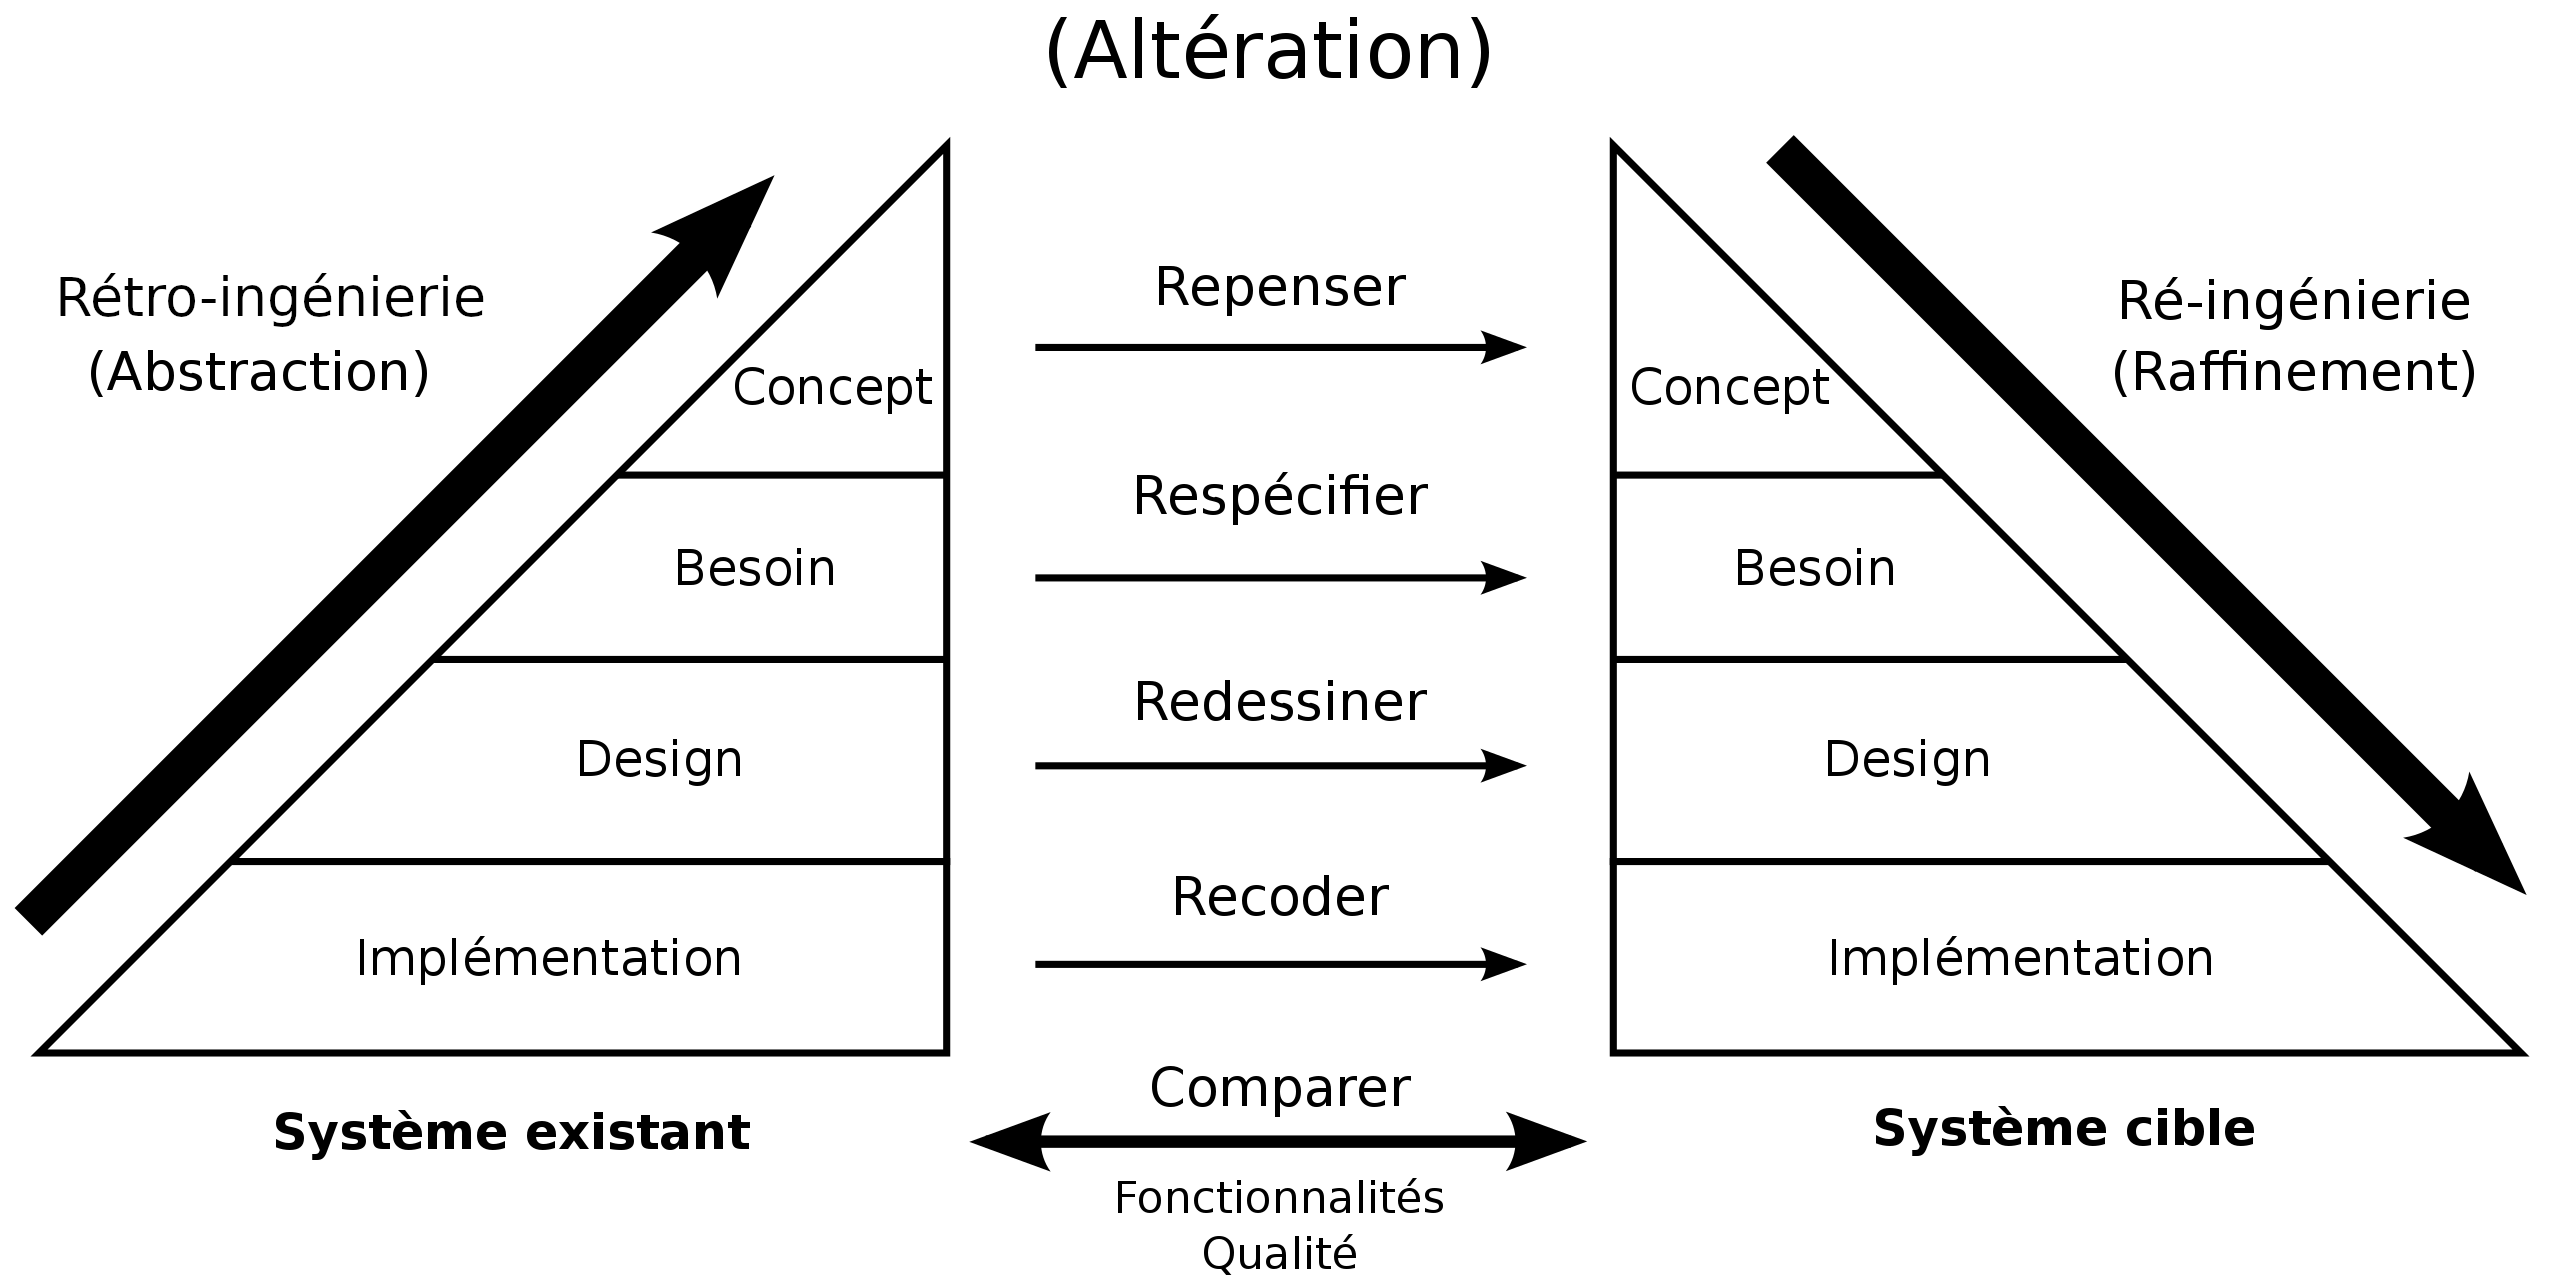
\includegraphics[width=5in]{images/Retroingenierie_-_Byrne.png}
\caption{Altération du code avec la rétro-ingénierie et la ré-ingénierie. Image modifiée~\cite{wikipedia_image_retroingenierie}}
\label{fig:retro_re_ing}
\end{figure}

Dans Figure~\ref{fig:exemple_gen_code_retro}, le code~\ref{lst:gen_code_retro_m} utilise la bibliothèque AST pour analyser l’arbre de syntaxe abstraite du code source. La difficulté avec la rétro-ingénierie est de savoir précisément ce qu’on cherche à extraire; il faut avoir un cas d’utilisation spécifique. Ici, le cas d’utilisation est la recherche d’un nœud de type expression qui contient des paramètres. L’avantage est de permettre de corriger des problèmes de qualité logicielle entre l’extraction d’information et la génération du code. Dans ce contexte, le résultat~\ref{lst:gen_code_retro_new_c} du code source original~\ref{lst:gen_code_retro_c} devient formaté en PEP8~\cite{python_pep8}.

\begin{figure}
\begin{lstlisting}[language=Python, upquote=true, caption={C mal formaté - fichier C.py de Figure~\ref{fig:exemple_gen_code_retro}}, label={lst:gen_code_retro_c}]
print(                     "Hello, World!"                         )
\end{lstlisting}

\begin{lstlisting}[language=Python, upquote=true, caption={M qui extrait µ$_C$ pour générer C.py de Figure~\ref{fig:exemple_gen_code_retro}}, label={lst:gen_code_retro_m}]
import ast

with open("C.py", "r") as f:
   code = f.read()

# Extraction du AST
tree = ast.parse(code)
node = tree.body[0]

if (
   isinstance(node, ast.Expr)
   and isinstance(node.value, ast.Call)
   and isinstance(node.value.func, ast.Name)
):
   # Si une expression executable de type function est trouve
   fct_arg = ""
   for arg in node.value.args:
       if isinstance(arg, ast.Str):
           # Cherche un parametre
           fct_arg = arg.s
           break
   # Template
   result = f"""{node.value.func.id}("{fct_arg}")\n"""

with open("C.py", "w") as f:
   f.write(result)
\end{lstlisting}

\begin{lstlisting}[language=Python, upquote=true, caption={C corrigé - fichier C.py de Figure~\ref{fig:exemple_gen_code_retro}}, label={lst:gen_code_retro_new_c}]
print("Hello, World!")
\end{lstlisting}
\caption{Exemple de technique de génération de code avec rétro-ingénierie d'un «Hello World»}
\label{fig:exemple_gen_code_retro}
\end{figure}

\subsection{Tester un générateur de code}

Il existe le test «Output comparison testing»~\cite{wikipedia_test_informatique} qui est le principe que le générateur de code crée du code (une sortie en texte lisible par l'humain) et que l'humain valide cette sortie textuelle.

Pour valider si le générateur utilise sa pleine capacité, il suffit de faire des tests de toutes les combinaisons de ses techniques de génération et d'utiliser un outil de couverture de code pour déterminer les lignes qui sont opérées.
